\documentclass{tufte-book}
\usepackage[utf8]{inputenc}
\usepackage{cite}
\usepackage{url}
\usepackage{hyperref}
\hypersetup{
colorlinks=true,
linkcolor=blue,
filecolor=red,
urlcolor=olive,
}

\usepackage{graphicx}
\usepackage{tikz}
\usetikzlibrary{decorations.pathmorphing}
\tikzset{snake it/.style={decorate, decoration=snake}}
\usetikzlibrary{decorations.markings}
\tikzset{middlearrow/.style={ decoration={markings, mark= at position 0.575 with {\arrow{#1}}, }, postaction={decorate} } }
\usepackage{amsmath,amssymb}
\usepackage{physics}
\usepackage{marginfix}

\setcounter{secnumdepth}{4}
\setcounter{tocdepth}{1}

\title{Notes on: Many Particle Physics --by D. Mahan}
\author{Meng Sun}

\newcommand{\bp}{\mathbf{p}}
\newcommand{\bq}{\mathbf{q}}
\newcommand{\bk}{\mathbf{k}}
\newcommand{\br}{\mathbf{r}}
\newcommand{\cd}{\mathcal{D}}
\newcommand{\cg}{\mathcal{G}}
\newcommand{\cf}{\mathcal{F}}


\begin{document}
\maketitle
\tableofcontents

\chapter{BASIC GROUP THEORY}

\section{Basic Definitions and Simple Example}
\textbf{Definition 1.1, Group} A set $\{G: a, b, c\dots\}$ is sai to form a group if there is an operaton called \textit{group multiplication}, which associates any given pair of elements $a, b \in G$ with a well-defined product $a \cdot b$ which is also an element of $G$, such that the following  condition are satisfied:
\begin{itemize}
  \item The operation $\cdot$ is associative, $a \cdot \left(b \cdot c\right) = \left(a\cdot b \right) \cdot c$for all $a, b, c \in G$;
  \item Among the elements of $G$, there is an element $e$, called the identity;
  \item For each $a \in G$, there is an inverse element, $a \cdot a^{-1}=e$.
\end{itemize}

\textrm{Example 1}: The $C_{2}$ group.
There are two group elements with the multiplication table in Tab.~\ref{tab:1-1}
\begin{table}
  \centering
  \begin{tabular}{c c}
    \hline
    e & a \\
    a & e \\
    \hline
  \end{tabular}
  \caption{Group Multiplication Table of $C_{2}$}
  \label{tab:1-1}
\end{table}
In physics, the spatial inversion transformation and identity form such a group.

\textit{Example 3}: There is one and only one three-element group called $C_{3}$ and the multiplication table is Tab.~\ref{tab:1-2}.
\begin{table}
  \centering
  \begin{tabular}{c c c}
    \hline \\
    e & a & b \\
    a & b & e \\
    b & e & a \\
    \hline
  \end{tabular}
  \caption{Group Multiplication Table of $C_3$}
  \label{tab:1-2}
\end{table}
Since $ab=e$ we conclude $b=a^{-1}$, we can denote the three elements by $\{e, a, a^{-1}\}$ with the requirement $a^{3}=e$.
Concrete examples of the the group $C_{3}$ are: the numbers $\left( 1, e^{i2\pi/3}, e^{-i2\pi/3}\right)$ with the usual rules of multiplication; the symmetry operations of the equilater trangle in the plane.

All these groups mentioned are examples of \textit{cyclic} group $C_{n}$ which have the general structure $\{e, a, a^{2}, \dots, a^{n-1}; a^{n}=e\}$ where $n$ can be any positive integer.

\textbf{Definition 1.2, Abelian group} An \textit{abelian group} $G$ is none for which the group multiplication is commutative.

\textbf{Definition 1.3, Order} The \textit{order} of a group is the number of elements of the group.

The cyclic groups $C_{n}$ described abover are all abelian.
Most interesting groups are not abelian.

\textrm{Example 4}: The simplist non-cyclic group is of order $4$.
It is usually called the \textit{dihedral group} denoted by $D_{2}$ with the multiplication table Tab.~\ref{tab:1-3}
\begin{table}
  \centering
  \begin{tabular}{c c c c}
    \hline
    e & a & b & c \\
    a & e & c & b \\
    b & c & e & a \\
    c & b & a & e \\
    \hline
  \end{tabular}
  \caption{Group Multiplication Table of $D_2$}
  \label{tab:1-3}
\end{table}

A visualize of this abelian group is by its association to a geometrical symmetry by considering the configuration of
Fig.~\ref{fig:1-1}.
\begin{figure}[h]
  \centering
  \begin{tikzpicture}
    \draw (0,0) -- (0,2) -- (4,2) -- (4,0) -- (0,0);
    \draw (0,1) -- (4,1);
    \draw (2,0) -- (2,2);
    \node [left] at (0,1) {$4$};
    \node [right] at (4,1) {$2$};
    \node [below] at (2,0) {$3$};
    \node [above] at (2,2) {$1$};
  \end{tikzpicture}
  \caption{A configuration with $D_2$ symmetry.}
  \label{fig:1-1}
\end{figure}
Applying the following tansformations on this figure: (i) leaving the figure unchanged; (ii) reflection about the vertical axis $(1,3)$; (iii) reflection about the horizontal axis $(2,4)$; and (iv) rotation of the figure in the plane around the center by $\pi$.
It is straightforward to check that the multiplication thable obtained through these geomentric constructions reproduces Tab.~\ref{tab:1-3}.

\section{Further Examples, Subgroups}
The smallest \textit{non-abelian group} is of order $6$.
It can be generated from the symmetry transformations of the geometric configuration of Fig.~\ref{fig:1-2}.
\begin{figure}[b]
  \centering
  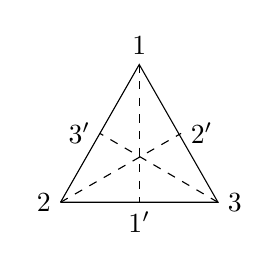
\begin{tikzpicture}
    \draw (0,0) -- (2,0) -- (1, 1.75) -- (0,0);
    \draw [dashed] (0,0) -- (1.531,0.875);
    \draw [dashed] (2,0) -- (0.5,0.875);
    \draw [dashed] (1,1.75) -- (1,0);
    \node [above] at (1,1.75) {$1$};
    \node [right] at (2,0) {$3$};
    \node [left] at (0,0) {$2$};
    \node [below] at (1,0) {$1'$};
    \node [right] at (1.531,0.875) {$2'$};
    \node [left] at (0.5,0.875) {$3'$};
  \end{tikzpicture}
  \caption{A configuration with $D_3$ symmetry}
  \label{fig:1-2}
\end{figure}
The operations are (1) the identity transformation, (ii) reflections about the axes $\left(1,1'\right)$ and so on and (iii) the rotations about the center by angles $\frac{2\pi}{3}$ and $\frac{4\pi}{3}$.
They form the \textit{dihedral group} $D_{3}$.
The reflecvtions interchange two fo the labels, leaving the remaining one unchanged, which we denote the oberation by $\left( 12\right)$.
For rotation counter-clockwise by $\frac{2\pi}{3}$ and $\frac{4\pi}{3}$ we deonte by $\left(321\right)$ and $\left(123\right)$ respectively.
One can see that there is a one-to-one correspondence between these symmetry transformations and the permutations of ther tree label whic form the permutation group $S_{3}$ in next section.
The group multiplication table is shown in Tab.~\ref{tab:1-4}.
\begin{table}
  \centering
  \begin{tabular}{c c c c c c}
    \hline \\
    $e$ & $\left(12\right)$ & $\left(23\right)$ & $\left(31\right)$ & $\left(123\right)$ & $\left(321\right)$ \\
    $\left(12\right)$ & $e$ & $\left(123\right)$ & $\left(321\right)$ & $\left(23\right)$ & $\left(31\right)$ \\
    $\left(23\right)$ & $\left(321\right)$ & $e$ & $\left(123\right)$ & $\left(23\right)$ & $\left(12\right)$ \\
    $\left(31\right)$ & $\left(123\right)$ & $\left(321\right)$ & $e$ & $\left(12\right)$ & $\left(23\right)$ \\
    $\left(123\right)$ & $\left(31\right)$ & $\left(12\right)$ & $\left(23\right)$ & $\left(321\right)$ & $e$ \\
    $\left(321\right)$ & $\left(23\right)$ & $\left(31\right)$ & $\left(12\right)$ & $e$ & $\left(123\right)$ \\
    \hline
  \end{tabular}
  \caption{Group Multiplication Table of $D_3$ or $S_3$}
  \label{tab:1-4}
\end{table}

\textbf{Definition 1.4, Subgroup} A subset $H$ of a group $G$ which forms a group under the same multiplication law as $G$ is said to form a \textit{subgroup} of $G$.

\textrm{Example 1} The group $S_{3}$ has four distinct subgroups consisting of the elements $\{e, \left(12\right)\}, \{e, \left(23\right)\}, \{e, \left(31\right)\}$ and $\{e, \left(123\right), \left(321\right)\}$ respectively.
The first three subgroups are identcal to the $C_{2}$ group.
The last one has the structure of $C_{3}$.
This can be seen by refering to the geometrical transformations in Fig.~\ref{fig:1-2}.

In many applications, the group elements carry labels which are continuous parameters.
These are \textit{continuous groups}.
Group of rotations in Euclidean spaces, and groups of continuous translations areprominent examples.
For later useage, we refere to the groups of ratiotions in space as $R\left(n\right)$ and the comined groups of rotations and translations in the same space as $E_{n}$.
The latter two are examples of \textit{Euclidean groups}.

Any set of invertible $n\times n$ matrices, which includes the unit matrix and which is closed under matrix multiplication, forms a \textit{matrix group}.
Important examples are:
\begin{itemize}
  \item the general \textit{linear group} $GL \left(n\right)$ consisting of all invertible $n\times n$ matrices;
  \item the \textit{unitary group} $U \left(n\right)$ consiting of unitary matrices, $U U^{\dagger} =1$;
  \item the \textit{special unitary group} $SU\left(n\right)$ consisting of unitary matrices with \textit{unit determinant} $\det{U}=1$;
  \item the \textit{orthogonal group} $O \left(n\right)$ consisting of real orthogonal matrics $OO^{T} = 1$.
\end{itemize}

These are examples of classical groups which occupy a central placew in group representation theory and have many applications in various branches of mathematics and physics.
Clearly, $SU\left(n\right)$ and $O\left(n\right)$ are subgroups of $U\left(n\right)$ which, in turn, is a subgroup of $GL\left(n\right)$.

\section{The Rearrangement Lemma and the Symmetric Group}
\textbf{Rearrangement Lemma:} If $p, b, c \in G$ and $pb = pc$ then $b=c$.

This result means: if $b$ and $c$ are distinct elements of $G$, then $pb$ and $pc$ are also distinct.
Therefore, if all the elements of $G$ are arranged in a sequencse and are multiplied on the left (right) by a given element $p$, the resulting squence is just a rearrangement of the original one.

Let us consider a finite group of order $n$, which is $\{g_{i}; i = 1,\dots, n\}$.
Multiply by $h\in G$ which is $g_{h_{i}} = hg_{i}$, then these $h_{i}$ are just the rearrangement of the label $i = 1, \dots, n$ and they must be distinct with each other due to the rearrangement lemma.

We introduce the \textit{group of permutations}.
An arbitrar permutation of $n$ objects wiht be denoted by
\begin{equation*}
  p =
  \begin{pmatrix}
    1 & 2 & 3 & \dots & n \\
    p_{1} & p_{2} & p_{3} & \dots & p_{n}
  \end{pmatrix}
\end{equation*}
The set of $n!$ permutations of $n$ objects form a group $S_{n}$ called the \textit{permutations group} or the \textit{symmetric group}.

A more compact and convenient notation for permution s is based on the \textit{cycle structure} which can be explained by example.
\begin{equation*}
  p =
  \begin{pmatrix}
    1 & 2 & 3 & 4 & 5 & 6 \\
    3 & 5 & 4 & 1 & 2 & 6
  \end{pmatrix}
\end{equation*}
We have the following replacement $1 \to 3 \to 4 \to 1$.
These three objects form a \textit{three-cycle} to tbe denoted by $\left(134\right)$.
Similarly, we have $\left(25\right)$ and $\left(6\right)$.
Then the \textit{cycle notation} $\left(134\right) \left(25\right) \left(6\right)$ uniquely specifies the permutation.
In this notation, the identity element consists of $n$ one-cycles,and inverse element is simply the same numbers in reverse order, i.e. $\left(p_{1}, p_{2}, \dots, p_{m} \right)^{-1} = \left(p_{m}, \dots, p_{2}, p_{1}\right)$.
We have already use this notation in Tab.~\ref{tab:1-4}.

\textbf{Definition 1.5, Isomorphism}: Two groups $G$ and $G'$ are said to be \textit{isomorphic} if there exists a one-to-one correspondence between their elements with preserves the law of group multiplication.
In other words, if $g_{i} \in G \leftrightarrow g_{i}' \in G'$ and $g_{1}g_{2} = g_{3}$ in $G$, gives $g_{1}'g_{2}'= g_{3}'$ in $G'$ and vice versa.

\textrm{Exampels}: (i) The group consisting of the numbers $\{\pm 1, \pm i \}$ with respect to the usual multiplication is isomorphic to the cyclic group $C_{4} = \{1, i, i^{2}=-1, i^{3} = -i; i^{4} = 1\}$.
(ii) The dihedral group $D_{3}$ is isomorphic to the symmetryc group $S_{3}$ defined above.

\textbf{Theorem 1.1, Cayley}: Every group $G$ of order $n$ is isomorphic to a subgroup of $S_{n}$.

\textrm{Example 1}: The cyclic group of order $3$, $\{C_{3}: e, a, b=a^{2}\}$ is isomorphic to the subgroup of $S_{3}$ consisting of the elements $\{e, \left(123\right), \left(321\right)\}$.

\textrm{Example 2}: The dihedral group $\{ D_{2}: e, a, b, c\}$ in Tab.~\ref{tab:1-3} is somorphic to the subgroup of $S_{4}$ consisting of the elements $\{ e, \left(12\right)\left(34\right), \left(13\right)\left(24\right), \left(14\right)\left(23\right)\}$.

An interesting general feature due to the Rearrangement Lemma is that no element other than the identity in a subgroup of $S_{n}$ which is isomorphic to a group of order $n$ in the specified way can contain one-cycles\footnote{The presence of a one-cycle means that a particular group element is uchanged upon left multiplication by another element which is not the identity. This contradicts the Rearrangement Lemma: $ba = a = e a$ then $b=e$.}
Furthermore, the cycles which do occur in any permutation associated with a given group element must alll be of the same length\footnote{If $g\in G$, have two cycle with differenct length $l_{1} < l_{2}$, then $g^{l_{1}}\in G$ contain one-cycle.}.
An interesting consequence of this result is that: if the order $n$ of a group is a prime number, then the corrsponding subgroup of $S_{n}$ can only contain unfactorized full $n-$fycles.
These correspond to elements of the cyclic group of order $n$.

\textbf{Theorem 1.2}: If the order $n$ of a group is a prime number, it must be isomorphic to $C_{n}$.

\section{Classes and Invariant Subgroups}
The elements of a group $G$ can be partitioned into conjugate classes and cosets.

\textbf{Definition 1.6} (Conjugate Elements): An element $b\in G$ is said to be \textit{conjugate} to $a \in G$ if there exists another group $p \in G$ such that $ b = p a p^{-1}$. We shal denote the conjugation relation by the symbol $\sim$.

Conjugation is an \textit{equivalence relation}: (i) each element is conjugate to itself $a \sim a$ (reflexive); (ii) if $a \sim b$ then $b \sim a$ (symmetric); and (iii) if $a \sim b$ and $b \sim c$, then $a \sim c$ (transitive).
It is well known that any equivalence relation provides a unique way to classify the elements of set.

\textbf{Definition 1.7} (Conjugate Class): Elements of a group which are conjugate to each other are said to form a (conjugate) class.

Each element of a group belongs to one and only one class.
The identity element forms a class all by itself.
For matrix groups, all elements in the same class are related to each other by some ``similarity transformation''.

\textrm{Example 1}: Elements of the permutation group $S_{3}$ can be divided into the following three classes: the identity $\zeta_{1} = e$, the calss of two-cycles $\zeta_{2} = \{\left(12\right), \left(23\right), \left(31\right)\}$, and the class of three-cycles $\zeta_{3}=\{\left(123\right),\left(321\right)\}$.
This example illustrates a general result for the general symmetric groups: permutations with the same cycle structure belong to the same class.

\textrm{Example 2}: In the group of 3-dimensionial rotations $R\left(3\right)$, let $R_{\hat{n}}\left(\psi\right)$ denote a rotation around the $\hat{n}$ axis by the angole $\psi$.
Then the rotations $\{R_{\hat{n}}; all \hat{n} \}$ for a given $\psi$ form a class.
This is because, for an arbitary $R$, $R \cdot R_{\hat{n}}\left(\psi\right) \cdot R^{-1} = R_{\hat{n'}}$ where $\hat{n'}$.

If $H$ is a subgroup of $G$ and $a \in G$, then $H' = \{ aha^{-1}; h \in H \}$ also form a subgroup of $G$.
$H'$ is said to be a \textit{conjugate subgroup} to $H$.
Clearly if $H$ and $H'$ are conjugate to each other, then they have the same number of elements.
One can also show that either $H$ and $H'$ are isomorphic or  they have only the identity element in common.

\textbf{Definition 1.8} (Invariant Subgroup): An \textit{invariant subgroup} $H$ of $G$ is one which is identical to all its conjuagate subgroups.

It is easy to see that a subgroup $H$ is invariant if and only if it contains elements of $G$ in gomplete classes.
It then follows that all subgroups of an abelian group are in invariant subgroup.

\textrm{Example}: For $S_{3}$, $\{e, \left(123\right), \left(321\right)\}$ form an invariant subgroup, but $\{e, \left(12\right)\}$ do not;

Let us examine the example explicitly.
$\{ e, \left(123\right), \left(321\right)\}$ is an invariant subgroup because it contains the identity and the entire class of three-cycles.
Every possible conjugate element of this set must be in these two classes, henec be in the orginal set.
For instance, $\left(12\right)\{e, \left(123\right),\left(321\right)\}\left(12\right)^{-1}=\{e, \left(321\right),\left(123\right)\}$, \ldots.
In contrast, $\{e,\left(12\right)\}$ is not an invariant subgroup because it only contains on of the three two-cycles.
One finds immediately that $\left(23\right)\{e, \left(12\right)\}\left(23\right)^{-1} = \{e, \left(31\right)\}$, hence one of the conjugate subgroups of $\{e, \left(12\right)\}$ is $\{e, \left(31\right)\}$ which is distinct from itself.

Every group $G$ has at lest two trivial invariant subgroups $\{e\}$ and $G$ itself.
If non-trival invariant subgroups exist, the full group can be ``simplified'' or ``factorized'' in ways to be discussed later.
Consequently, it is natural to adopt the following definition.

\textbf{Definition 1.9} (Simple and Semi-simple Groups): A group is \textit{simple} if it does not contain any non-trival invariant subgroup.
A group is \textit{semi-simple} if it does not contain any abelian invariant subgroup.

\textrm{Examples}: (i) The cyclic groups $C_{n}$ with $n=$prime numberare simple groups; (ii) $C_{n}$ with $n=$non-prime number are neither simple nnor semi-simple.
For example, $C_{4}= \{e,a,a^{2},a^{3}\}$ has a subgroup $\{e, a^{2}\}$ which is invariant and abelian;
(iii) The group $S_{3}$ is neither simple nor semi-simple, it has an abelian invariant group $\{e, \left(123\right), \left(321\right)\}$;
(iv) The three-dimensional rotation group $SO\left(3\right)$ is simple, but the two-dimensional rotation group is not.

\section{Cosets and Factor (Quotient) groups}
\textbf{Definition 1.10} (Cosets): Let $H=\{h_{1},h_{2},\dots\}$ be a subgroup of $G$ and let $p$ be and element of $G$ (one which is not in $H$), then the set of elements $pH=\{ph_{1}, ph_{2},\dots\}$ is called a \textit{left coset} of $H$.
Similarly, $Hp= \{h_{1}p,h_{2}p,\dots\}$ is a \textit{right coset} of $H$.

Everythin discussed concerning the left coset has its counterpart for right cosets.
Aside from $H$ itself, cosets are not subgroups.
Each coset has exactl the same number of distinct elements as $H$, as a consequence of the rearrangement lemma.

\textbf{Lemma}: Two left cosets of a subgroup $H$ either coincide completely, or else have no elements in common at all.

Given a subgroup $H$ of order $n_{H}$, the distinct left cosets of $H$ partition the elements of the full group $G$ into disjoint sets of $n_{H}$ each.

\textbf{Theorem 1.3} (Lagrange): The order of finite group must be an integer multiple of the order of any of its subgroups.

\textrm{Examples}: Consider the permutation group $S_{3}$: (i) the subgroup $\{H_{1} : e, \left(123\right), \left(321\right)\}$ has one coset $\{M: \left(12\right),\left(23\right),\left(31\right)\}$; (ii) The subgroup $\{H_{2} : e, \left(12\right)\}$ has tow left cosets: $\{M_{1}: \left(23\right),\left(321\right)\}$, obtained from $H_{2}$ by multiplication with either $\left(23\right)$ or $\left(321\right)$, and $\{M_{2}: \left(31\right),\left(123\right)\}$, obtained from $H_{2}$ by multiplication with either $\left(31\right)$ or $\left(123\right)$. We illustrate schematically the partioning of the elements of $S_{3}$ according to cosets and classes in Fig.~\ref{fig:1-3}.
\begin{marginfigure}
  \centering
  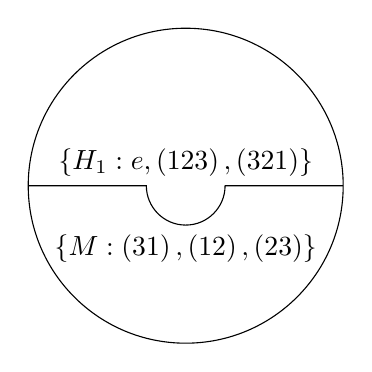
\begin{tikzpicture}
    \draw (0,0) circle [radius=2];
    \draw (2,0) -- (0.5,0) arc [radius=0.5, start angle = 0, end angle = -180] -- (-2,0);
    \node [above] at (0,0) {$\{H_{1}: e, \left(123\right),\left(321\right)\}$};
    \node [below] at (0,-0.5) {$\{M: \left(31\right), \left(12\right), \left(23\right)\}$};
  \end{tikzpicture}
  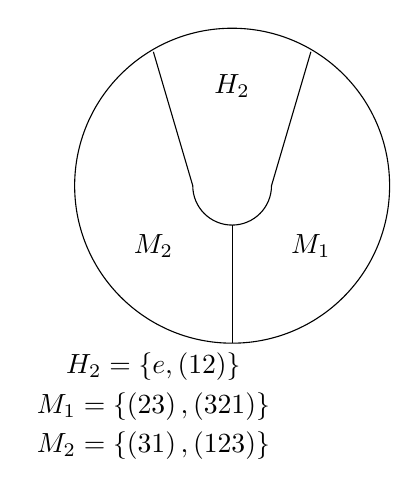
\begin{tikzpicture}
    \draw (0,0) circle [radius=2];
    \draw (1,1.7) -- (0.5,0) arc [radius=0.5, start angle = 0, end angle = -180] -- (-1,1.7);
    \draw (0,-2) -- (0,-0.5);
    \node [above] at (0,1) {$H_{2}$};
    \node [below] at (-1,-0.5) {$M_{2}$};
    \node [below] at (1,-0.5) {$M_{1}$};
    \node [below] at (-1,-2) {$H_{2}= \{e, \left(12\right)\}$};
    \node [below] at (-1,-2.5) {$M_{1}=\{\left(23\right), \left(321\right)\}$};
    \node [below] at (-1,-3) {$M_{2}=\{\left(31\right), \left(123\right)\}$};
  \end{tikzpicture}
  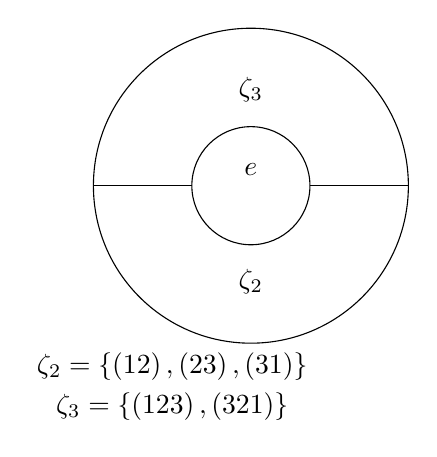
\begin{tikzpicture}
    \draw (0,0) circle [radius=2];
    \draw (0,0) circle [radius=0.75];
    \draw (0.75,0) -- (2,0);
    \draw (-2,0.0) -- (-0.75, 0.0);
    \node [above] at (0,0) {$e$};
    \node [below] at (0,1.5) {$\zeta_{3}$};
    \node [above] at (0,-1.5) {$\zeta_{2}$};
    \node [below] at (-1,-2) {$\zeta_{2}=\{\left(12\right), \left(23\right), \left(31\right)\}$};
    \node [below] at (-1,-2.5) {$\zeta_{3} = \{\left(123\right), \left(321\right)\}$};
  \end{tikzpicture}
  \caption{(a) left cosets of $H_1$ (b) left cosets of $H_2$ (c) classes of $S_3$.}
  \label{fig:1-3}
\end{marginfigure}

The cosets of invariant subgrous are particularly simple and useful.
First, if $H$ is an invariant subgroup, its left cosets are also right cosets\footnote{If $H$ is invariant subgroup $p H p^{-1} = H$, this implies $pH = Hp$.}.
The partitioning of the elements of the full group $G$ into cosets is unique, and a ``factorization'' of $G$ based on this partioning becomes natural.
Let us consider the cosets of an invariant subgroup $H$ as elements of a new group.
The multiplication of two cosets $pH$ and $qH$ is defined as the coset consisting of all products $ph_{i}qh_{j} = \left(pq\right)h_{k}$, where $h_{k} = \left(q^{-1} h_{i} q \right) h_{j} \in H$ provided $h_{i},h_{j} \in H$ and $p,q \in G$.
Since $pH \cdot qH = \left(pq\right) H$, it becomes obvious that (i) $H=eH$ plays the role of the iendtity element; (ii) $p^{-1}H$ is the inverse of $pH$; and (iii) $pH \left(qH \cdot rH \right) = \left(p H \cdot qH \right) \cdot rH = \left(pqr\right) H$.

\textbf{Theorem 1.4} If $H$ is an invarian subgroup of $G$, the set of cosets endowed with the law of multiplication $pH \cdot qH = \left(pq\right)H$ form a group, called the \textit{factor or quotient} group of $G$.
The factor group is denote by $G/H$, it is of order $n_{G}/n_{H}$.

\textrm{Exampel 1}: Consider the inveriant subgroup $H= \{e, a^{2}\}$ of the cyclic group $C_{4}$.
$H$ and coset $M=\{a, a^{3}\}$ form the factor group $C_{4}/H$.
Applying the rule of multiplication of cosets described above, it is straight forward to verify that $HM = M = MH$, $HH = H$, and $MM = H$.
We see that both the subgroup $H$ and the factor group $C_{4}/H$ are of order $2$ and are isomorphic to $C_{2}$.

\textrm{Example 2}: In the case of the permutation group $S_{3}$, $H=\{e, \left(123\right), \left(321\right)\}$ represents an invariant subgroup in Fig.~\ref{fig:1-3} and Tab.~\ref{tab:1-4}.
$G/H$ consists of two elements: $H$ and $M=\{\left(12\right), \left(23\right), \left(31\right)\}$.
We have: $HM= H\cdot \left(ij\right)H= \left(ij\right) H = M = MH$, and $HH= MM = H$.
Therefor, $G/H$ is also isomorphic to the cyclic group of order $2$, $C_{2}$.

\textrm{Example 3}: Consider the discrete translation group $T^{d}=\equiv \Gamma$ and one of its invariant subgroups $\Gamma_{m}$.
The cosets are $\Gamma_{m}$, $T\left(1\right) \Gamma_{m}$, $T\left(2\right) \Gamma_{m}$, \ldots, $T\left(m-1\right) \Gamma_{m}$ and $T\left(m\right) \Gamma_{m} = \Gamma_{m}$.
Hence the factor group $\Gamma/\Gamma_{m}$ is isomorphic to the cyclic group $C_{m}$.
Infinite groups, such as this one, do not behave exactly like finite ones.
For instance, $\Gamma$  and $\Gamma_{m}$ are, in fact, isomorphic to each other even though $\Gamma/\Gamma_{m}$ is non-trival.

\textrm{Example 4}: We state without proof that the translations in $3-$dimensional space form a invariant subgroup of the Euclidean group $E_{3}$; and the factor group is isomrophic to the group of rotations.
This fact forms the basis of important techniques to analyze the Euclidean group and its generalization to $4-$dimensional spacetime---the Poincar\'{e} group.

\section{Homorphisms}
\textbf{Definition 1.11} (homomorphism): A \textit{homomorphism} from a group $G$ to another group $G'$ is a mapping (not necessarily one-to-one) which preserves group multiplication.
In other words, if $g_{i} \in G \to g_{i} \to g_{i}' \in G'$ and $g_{1}g_{2}=g_{3}$, then $g_{1}'g_{2}'=g_{3}'$.

Clearly, isomorphism is a special case of homomorphism.
\begin{figure}
  \centering
    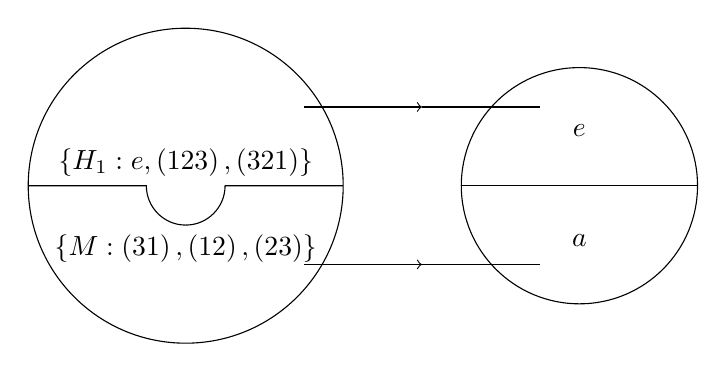
\begin{tikzpicture}
    \draw (0,0) circle [radius=2];
    \draw (2,0) -- (0.5,0) arc [radius=0.5, start angle = 0, end angle = -180] -- (-2,0);
    \node [above] at (0,0) {$\{H_{1}: e, \left(123\right),\left(321\right)\}$};
    \node [below] at (0,-0.5) {$\{M: \left(31\right), \left(12\right), \left(23\right)\}$};
    \draw (5,0) circle [radius=1.5];
    \draw [->] (1.5,1) -- (3,1);
    \draw (3,1) -- (4.5,1);
    \draw [->] (1.5,-1) -- (3,-1);
    \draw (3,-1) -- (4.5,-1);
    \draw (3.5, 0) -- (6.5, 0);
    \node [above] at (5,0.5) {$e$};
    \node [below] at (5,-0.5) {$a$};
  \end{tikzpicture}
  \caption{Homomorphism from $S_3$ to $C_2$.}
  \label{fig:1-4}
\end{figure}

\textrm{Example}:  The mapping from $S_{3}$ to $C_{2}$ depicted in Fig.~\ref{fig:1-4} is a homomorphism.
This follows from the fact that the product of any two element s from $H$ or from $M$ results in an element in H, whereas the product of one element from $H$ with on element from $M$ results in an element in $M$.
This example illustrates the general result that if $G$ has an invariant subgroup $H$, then there exists a natural homomorphism from $G$ to the factor group $G/H: g\in G \to gH \in G/H$.
Group multiplication is preserved b definition.
This result can be turned around to ield the following interesting theorem.

\textbf{Theorem 1.5}: Let $f$ be a homomorphism form $G$ to $G'$.
Denote by $K$ the set of all elements of $G$ whare are mapped to the identity element of $G'$, i.e. $K= \{a \in G; f(a) = e' \in G'\}$.
Then $K$ forms an invariant subgroup of $G$.
Furthermore, the factor group $G/K$ is isomorphic to $G'$.

\section{Direct Products}
Many physically useful symmetry groups are direct products of simpler groups.
When this is the case, it suffices to know the structure and the representations of the smaller groups.

\textbf{Definition 1.12} (Direct Product Group): Let $H_{1}$ and $H_{2}$ be subgroups of a group $G$ with the following properties: (i) every element of $H_{1}$ commutes with any element of $H_{2}$, i.e. $h_{1}h_{2} = h_{2} h_{1}$ for $\forall h_{1} \in H_{1}$ and $\forall h_{2}\in H_{2}$; and (ii) every element $g$ for $G$ can be written uniquely as $g=h_{1}h_{2}$ where $h_{1}\in H_{1}$ and $h_{2}\in H_{2}$.
In this case, $G$ is said to be the direct product of $H_{1}$ and $H_{2}$; symbolically, $G= H_{1}\otimes H_{2}$.

\textrm{Example 1}: Consider the group $C_{6}$ with elements $\{e = a^{6}, a, a^{2}, a^{3}, a^{4}, a^{5}\}$, and the subgroups $H_{1} = \{e, a^{3}\}$ and $H_{2} = \{e, a^{2}, a^{4}\}$.
Cirterion (i)is trivally satisfied because the group is abelian, and (ii) can be verified by $e=ee$, $a = a^{3} a^{4}$ and so on.
Since $H_{1}$ and $H_{2}$ are isomorpism to $C_{2}$ and $C_{3}$, i.e. $H_{1} \simeq C_{2}$ and $H_{2} \simeq C_{3}$, we have $C_{6} \simeq C_{2} \otimes C_{3}$.

If $G= H_{1}\otimes H_{2}$, then both $H_{1}$ and $H_{2}$ must be invariant subgroups of $G$.
\footnote{If $g=h_{1}h_{2}\in G$, and $h_{1}, a \in H_{1}$, $h_{2}\in H_{2}$. Then $g a g^{-1} = h_{1}h_{2} a h_{2}^{-1} h_{1}^{-1} = h_{1} a h_{1}^{-1} \in H_{1}$ for all $g$ and $a$.}
Now, we can form the quotient group $G/H_{2}$ and prove that, $G/H_{2} \simeq H_{1}$.
However, the converse to the above is not true!
Let $H$ be an invariant subgroup of $G$ and $H'= G/H$.
It does not follow that $G = H \otimes H'$.


%%% Local Variables:
%%% mode: latex
%%% TeX-master: "main"
%%% End:

\chapter{GROUP REPRESENTATIONS}

\section{Representations}
\textbf{Definition 2.1} (Representations of a Group): If there is a homomorphism from a group $G$ to a group operatures $U\left(G\right)$ on a linear vector space $V$, we say that $U\left(G\right)$ forms a \textit{representation} of the group $G$.
The \textit{dimension of the representations} is the dimension of the vector space $V$.
A representation is said to be \textit{faithful} if the homomorphism is alo an isomorphism.
A \textit{degenerate representation} is one which is not faithful.

To be more specific: the representation is a mapping
\begin{equation*}
  g \in G \xRightarrow[above]{U} \left(g\right)
\end{equation*}
where $U\left(g\right)$ is an operator on $V$, such that
\begin{equation}
  \label{eq:2.1-1}
  U\left(g_{1}\right) U\left(g_{2}\right) = U \left(g_{1} g_{2}\right)
\end{equation}
i.e., the representation operators satisfy the same rules of multiplication as the original group elements.

Consider the case of a finite-dimensional representation.
Choose a set of basis vectors on $V$.
The operators $U\left(g\right)$ are then realized as $n\times n$ matrices $D\left(g\right)$ as follows\footnote{where $j$ is the row index and $i$ is the column index}:
\begin{equation}
  \label{eq:2.1-2}
 U\left(g\right) \ket{e_{i}} = \ket{e_{j}} D\left(g\right)^{j}_{i}, ~ ~ ~ g \in G.
\end{equation}
And from Eq.~\eqref{eq:2.1-1}, we have
\begin{equation}
  \label{eq:2.1-3}
 D\left(g_{1}\right) D\left(g_{2}\right) = D\left(g_{1}g_{2}\right)
\end{equation}
And since $D\left(G\right)$ satisfy the same algebra as $U\left(G\right)$, the group of matrices $D\left(G\right)$ forms a \textit{matrix representation} of $G$.

\textrm{Example 1}: The trivial $1-$dimenional representation for every group $G$.
Let $V=C$, and $U\left(g\right) = 1$ for all $g \in G$.
Then $g\in G \longrightarrow 1$ forms a representation.

\textrm{Example 2}: Let $G$ be a group of matrices, $V=C$, and $U\left(g\right) =\det g$.
This define non-trivial one-dimenional representation since $\det g_{1} \det g_{2} = \det g_{1}g_{2}$.

\textrm{Example 4}: Let $G$ be the dihedral group $D_{2}$ consisting of $e$ (identity), $h$ (reflection about the $Y-$axis), $v$ (reflection about the $X-$axis), and $r$ (rotation by $\pi$ around the origin) as described at Tab.~\ref{tab:1-3} and Fig.~\ref{fig:1-1}.
Let $V_{2}$ be the two-dimensional Euclidean space with basis vector $\left(\hat{e}_{1}, \hat{e}_{2}\right)$.
By referring to Fig.~\ref{fig:2-1} and making use of the definition Eq.~\eqref{eq:2.1-2}, we easily infer
\begin{equation}
  \label{eq:2.1-4}
  D\left(e\right) =
  \begin{bmatrix}
    1 & 0 \\
    0 & 1
  \end{bmatrix}
  D\left(h\right) =
  \begin{bmatrix}
    -1 & 0 \\
    0 & 1
  \end{bmatrix}
  D\left(v\right) =
  \begin{bmatrix}
    1 & 0 \\
    0 & -1
  \end{bmatrix}
  D\left(r\right) =
  \begin{bmatrix}
    -1 & 0 \\
    0 & -1
  \end{bmatrix}
\end{equation}
It is straightforward to very that the mapping $g\longrightarrow D\left(g\right)$ is a homomorphism, hence these matrices form a $2-$dimensional representation of the $D_{2}$ group.
\begin{figure}
  \centering
  \begin{tikzpicture}
    \draw [<->] (-2,0) -- (2,0);
    \draw [<->] (0,-2) -- (0,2);
    \draw [dashed] (0,0) circle [radius=2];
    \node [right] at (2,0) {$\hat{e}_{1}, ~ v\hat{e}_{1}$};
    \node [above] at (0,2) {$\hat{e}_{2}, ~ h\hat{e}_{2}$};
    \node [left] at (-2,0) {$r\hat{e}_{1}, ~ h\hat{e}_{1}$};
    \node [below] at (0,-2) {$v\hat{e}_{2}, ~ r\hat{e}_{2}$};
  \end{tikzpicture}
  \caption{$D_2$ transformations}
  \label{fig:2-1}
\end{figure}

\textrm{Example 5}: Let $G$ be the group of continuous rotations in a plane around origin $O$, $G=\{R\left(\phi\right), 0\leq \phi \leq 2\pi\}$.
Let $V_{2}$ be the two-dimensional Euclidean space, since
\begin{align}
  \label{eq:2.1-5}
  \hat{e}_{1}' &= \hat{e}_{1} \cos \phi + \hat{e}_{2} \sin \phi \\
  \hat{e}_{2}' &= -\hat{e}_{1} \sin \phi + \hat{e}_{2} \cos \phi \nonumber
\end{align}
we have
\begin{equation}
  \label{eq:2.1-6}
  D\left(\phi\right) =
  \begin{bmatrix}
    D_{1}^{1}=\cos \phi & D_{1}^{2}=-\sin \phi \\
    D_{2}^{1}=\sin \phi & D_{2}^{2}=\cos \phi
  \end{bmatrix}
\end{equation}
Since according Eq.~\eqref{eq:2.1-2}, $U \ket{e_{1}} = \ket{e_{1}} D\left(\phi\right)_{1}^{1}+ \ket{e_{2}} D\left(\phi\right)_{1}^{2}$.
However, if $\mathbf{x}$ is an arbitrary vector in $V_{2}$, $\mathbf{x} = \hat{e}_{j} x^{j}$, then
\begin{align}
  \label{eq:2.1-7}
  \mathbf{y} &= U\left(\phi\right) \mathbf{x} = \hat{e}_{j} y^{j} \\ \nonumber
  y^{j} &= D\left(\phi\right)^{j}_{i} x^{i} \\ \nonumber
  \begin{bmatrix}
    y^{1} \\
    y^{2}
  \end{bmatrix}
  &=
  \begin{bmatrix}
  \cos \phi & -\sin \phi \\
  \sin \phi & \cos \phi
  \end{bmatrix}
  \begin{bmatrix}
  x^{1}\\
  x^{2}
  \end{bmatrix}
\end{align}

As we can see, different groups may be realized on the same vector space.
Here, the $2-$dimensional Euclidean space $V_{2}$ is seen to provide representations for the two finite groups $D_{2}$, $D_{3}$ as well as the continuous group $R\left(2\right)$

\textrm{Example 7}: Let $V_{f}$ be te space of complex-valued linear homogeneous founctions $f$ of two real varibales $\left(x,y\right)$:
\begin{equation}
  \label{eq:2.1-8}
  f\left(x,y\right) = a x + by
\end{equation}
where $\left(a,b\right)$ are arbitary complex coefficients.
Interpret $\left(x,y\right)$ as the components of a vector $\mathbf{x}$ in a $2$-dimenional Euclidean space $V_{2}$.
Then the group operations from previos examples will induce the following transformation in the function space $V_{f}$
\begin{equation}
\label{eq:2.1-9}
f \xRightarrow{g \in G} f'\left(x^{1},x^{2}\right) \equiv f \left(x'^{1},x'^{2}\right)
\end{equation}
where $\mathbf{x}' = U\left(g^{-1}\right) \mathbf{x}$.
It is straightforward to show that the mapping defined by Eq.~\eqref{eq:2.1-9} is a homomorphism; for if $g" g' = g$ then
\begin{align}
\label{eq:2.1-10}
f \xRightarrow{g'} f' ~ ~ ~ f' \left(\mathbf{x}\right) &= f \left[ U\left(g'\right)^{-1} \mathbf{x} \right] \\ \nonumber
f' \xRightarrow{g"} f" ~ ~ ~ f"\left( \mathbf{x} \right) &= f' \left[ U\left(g"\right)^{-1} \right] = f \left[U\left(g'\right)^{-1} U\left(g"\right)^{-1} \mathbf{x} \right] \\ \nonumber
  &= f\left[U\left(g"g'\right)^{-1} \mathbf{x}\right] = f\left[ U\left(g\right)^{-1} \mathbf{x}\right]
\end{align}
Therefore, the set of transformation defined by Eq.~\eqref{eq:2.1-9} forms a representation of the group $G$.

\textbf{Theorem 2.1:} (i) If the group $G$ has a non-trivial invariant subgroup $H$, then any representation of the factor group $K=G/H$ is also a representaion of $G$.
This representaion must be degenerate; (ii) Conversely, if $U \left( G \right)$ is a degenerate representation of $G$, then $G$ has at least one invariant subgroup $H$ such that $U \left( G \right)$ defines a faithful representation of the factor group $G/H$.

A immediate corollay of this theorem is that all representations of simple groups are faithful.

\section{Irreducible, Inequivalent Representations}
The first type of redundacy is due to similarity transformation.

\textbf{Definition 2.2} (Equivalence of Representations): Two representations of a group $G$ related by a similarity transfromation are said to be equivalent.

By seeking characterizations of the representation which are invariant under similarity transfomations, we can tell the two representations are equivalant or not.
The trace $\tr A$ and determinant $\det A$ are two characterizations which are independent of the choice of the base.

\textbf{Definition 2.3} (Characters of a Representation): The \textit{character} $\chi \left( g \right)$ of $g \in G$ in a represenation $U \left( G \right)$ is defined to be $\chi \left( g \right) = \Tr U \left( g \right)$.
All group elements in a given class of $G$ have the same characters, becase $\Tr D \left( p \right) D \left( g \right) D \left( p^{-1} \right)= \Tr D \left( g \right)$.
Therefor, the group character is a function of the class-label only.

A second type of redundacy concerns direct sum representations.

\textbf{Definition 2.4} (Invariant Subspace): Let $U \left( G \right)$ be a representation of $G$ on the vector space $V$, and $V_{1}$ be a subspace of $V$ with the property that $U \left( g \right) \ket{x} \in V_{1}$ for all $\mathbf{x} \in V_{1}$ and $g \in G$.
$V_{1}$ is siad to be an \textit{invariant subspace} of $V$ with repsect ot $U \left( G \right)$.
An invariant subspace is \textit{mimimal} or \textit{proper} if it does not contain any non-trival invariant subspace with respect ot $U \left( G \right)$.

Examples of trivial invariant subspaces of $V$ with respect to $U \left( G \right)$ are: (i) the space $V$ itself, and (ii) the subspace consisting only of the null vector.

\textbf{Definition 2.5} (Irreducibel Representations): A representation $U \left( G \right)$ on $V$ is \textit{irreducible} if there is no non-trivial invariant subspace in $V$ with respect to $U \left( G \right)$.
Otherwise, the representation is \textit{reducible}.
In latter case, if the orthogonal complement\footnote{If $V_{1}$ is a subspace of $V$, the orthogonal complement of $V_{1}$ consists of all vectors in $V$ which are orthogonal to very vector in $V_{1}$. For finite-dimensional vector spaces, at least, the orthogonal complement of $V_{1}$ also forms a subspace, called $V_{2}$, then we have $V = V_1 \oplus V_2$.}of the invariant subspace is also invariant with respect to $U \left( G \right)$, then the represenation is said to be \textit{fully reducible or decomposable.}

\textrm{Example 1}: Consider the action of the dihedral group $D_2$ on the $2-$dimensional Euclidean space $V_2$ as described in Fig.~\ref{fig:2-1} and Eq.~\eqref{eq:2.1-4}.
The $1-$dimensional subspace spanned by $\hat{e}_1$ is invariant under all four group operations, $D_2 \left( g \right) \hat{e}_1 = \pm \hat{e}_1$.
The same is true for the subspace spaned by $\hat{e}_2$.
Thus the $2-$dimensional representation of the group given by Eq.~\eqref{eq:2.1-4} is therefore a reducible representation.

\textrm{Example 2}: The $1-$dimensional subspace spanned by $\hat{e}_{1}$ or $\hat{e}_2$ is not invariant under the group $\mathbf{R} \left( 2 \right)$.
However, if we form the following linear combinations of vectors,
\begin{equation}
  \label{eq:2.2-1}
 \hat{e}_{\pm} = \frac{1}{\sqrt{2}} \left( \mp \hat{e}_1 - i \hat{e}_2 \right)
\end{equation}
it is straightforward to show that:
\begin{align}
  \label{eq:2.2-2}
  U \left( \phi \right) \hat{e}_+ &= \hat{e}_+ e^{-i\phi} \\ \nonumber
  U \left( \phi \right) \hat{e}_- &= \hat{e}_- e^{i\phi}
\end{align}
Therefore, the $1-$dimensional spaces spanned by $\hat{e}_{\pm}$ are individually invariant under the rotation group $R \left( 2 \right)$.
The $2-$dimensional representation given by Eq.~\eqref{eq:2.1-6} can be simplified if we make a change of basis to the eigenvectors $\hat{e}_{\pm}$.
In this new basis,
\begin{equation}
  \label{eq:2.2-3}
  D' \left( \phi \right) =
  \begin{bmatrix}
    e^{-i\phi} & 0 \\
    0 & e^{i\phi}
  \end{bmatrix}
\end{equation}
The new matrices can be obtained form the old one in Eq.~\eqref{eq:2.1-6} by a similarity transformation which is defined by Eq.~\eqref{eq:2.2-1}.

Let us look at the general matrix form of a reducible representation.
If $V_1$ is an $n_1-$dimensional invariant subspace with respect to $U \left( G \right)$, we can always choose a set of basis vectors in $V$ such that the first $n_1$ vectors are in $V_1$.
Since, for all $g\in G$
\begin{equation}
 U \left( g \right) \ket{e_i} = \ket{e_j} D \left( g \right)^j_i \in V_1 ~ ~ ~ \text{for}~ i= 1, \dots, n_{1} \nonumber
\end{equation}
we conclude that $D \left( g \right)_i^j = 0$ for $i=1, \dots, n_1$ and $j= n_1+1, \dots, n$.
Therefor, the matrix representation is of the form
\begin{equation}
  \label{eq:2.2-4}
  D \left( g \right) =
  \begin{bmatrix}
    D_1 \left( g \right) & D' \left( g \right) \\
    0 & D_2 \left( g \right)
  \end{bmatrix}
\end{equation}
If $D \left( g \right)$ and $D \left( g' \right)$ are both of this form, then the product $D \left( gg' \right)$ is also of this form, and that $D_i \left( gg' \right) = D_i \left( g \right) D_i \left( g' \right)$ for $i=1,2$.
Thus, all esential properties of $D \left( G \right)$ are already contained in the representations $D_i \left( G \right)$.

We see that if $U \left( G \right)$ is a representation of the group $G$ on $V$ and $V^{\mu}$ is an invariant subspace of $V$ respect to $G$, then by restricing the action of $U \left( G \right)$ to $V^{\mu}$, we obtain a lower-dimension representation $U^{\mu} \left( G \right)$.
If the subspace $V^{\mu}$ cannot be further reduced, $U^{\mu} \left( G \right)$ is an irreducible represenation, and we say that $V^{\mu}$ is a \textrm{proper or irreducible invariant subspace} with respect to $G$.

\section{Unitary Representations}
\textbf{Definition 2.6} (Unitary Representation): If the group representation space is a inner product space, and if the operators $U \left( g \right)$ are unitary for $g \in G$, then the representation $U \left( G \right)$ is said to be a \textit{unitary representation}.

Because symmetry transformation are naturally associated with unitary operators, unitary representations play a cnetral role in studying symmetry groups.

\textbf{Theorem 2.2:} If a unitary representation is reducible, then it is alos decomposable i.e., fully reducible.

\textbf{Theorem 2.3:} Every representation $D \left( G \right)$ of a finite group on an inner product space is equivalent to a unitary representation, i.e., there exist a similar transformation such that $S D \left( g \right) S^{-1}$ is unitary.






%%% Local Variables:
%%% mode: latex
%%% TeX-master: "main"
%%% End:

\chapter{Formalism}

\chapter{Quantum mecahnics in three dimensions}
\section{Schr\"odinger equation in spherical coordinates}
The generalization to three dimsnison is straightforward.
\begin{equation}
  \label{eq:4-1}
  i\hbar \frac{\partial \Psi}{\partial t} = - \frac{\hbar^{2}}{2m} \nabla^{2} \Psi + V\Psi
\end{equation}
where the \textbf{Laplacion} is
\begin{equation}
  \label{eq:4-2}
  \nabla^{2} \equiv \frac{\partial^{2}}{\partial x^{2}} + \frac{\partial^{2}}{\partial y^{2}} + \frac{\partial^{2}}{\partial z^{2}}
\end{equation}
in cartesian coordinates.
With the separation of the variables the general solution gives
\begin{equation}
  \label{eq:4-3}
  \Psi \left( \mathbf{r},t \right) = \sum c_{n} \psi_{n} \left( \mathbf{r} \right) e^{-i E_{n}t/\hbar}.
\end{equation}

\subsection{Separation of variables}
Typically, the potential is a function only of the distance from the origin.
In that case it is natural to adopt \textbf{spehrical coordinates}, as shown in Fig.~\ref{fig:4-1}, the Laplacian takes the form for our time-independent Schr\"odinger equation
\begin{equation}
  \label{eq:4-4}
  \nabla^{2} = \frac{1}{r^{2}} \frac{\partial }{\partial r} \left( r^{2} \frac{\partial}{\partial r} \right) + \frac{1}{r^{2}\sin\theta} \frac{\partial}{\partial \theta} \left( \sin\theta \frac{\partial}{\partial \theta} \right) + \frac{1}{r^{2} \sin^{2} \theta} \left( \frac{\partial^{2}}{\partial \phi^{2}} \right).
\end{equation}
\begin{figure}[h]
  \centering
  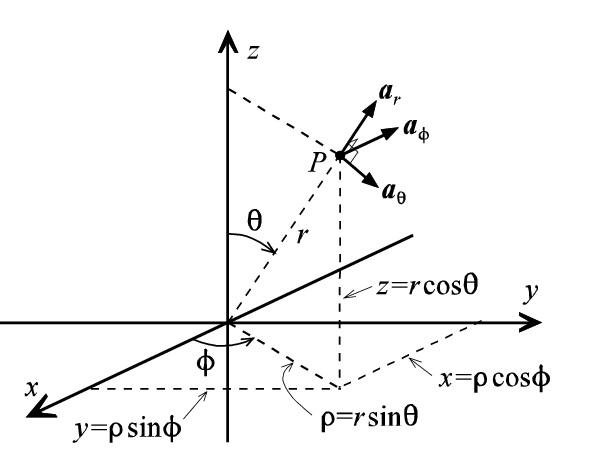
\includegraphics[width=0.45\textwidth]{fig/fig4-1.png}
  \caption{Spherical coordinates.}
  \label{fig:4-1}
\end{figure}

We begin by looking for solutions that are separable into products
\begin{equation}
  \label{eq:4-5}
  \psi \left( r,\theta,\phi \right) = R \left( r \right) Y \left( \theta, \phi \right).
\end{equation}
With this ansatz, we have
\begin{equation}
  \label{eq:4-6}
  \left\{ \frac{1}{R} \frac{\dd}{\dd r} \left( r^{2} \frac{\dd R}{\dd r} \right) - \frac{2mr^{2}}{\hbar^{2}} \left[ V \left( r \right) -E \right] \right\}  + \frac{1}{Y} \left\{  \frac{1}{\sin\theta} \frac{\partial}{\partial \theta} \left( \sin\theta \frac{\partial Y}{\partial \theta} \right) + \frac{1}{ \sin^{2} \theta} \frac{\partial^{2} Y}{\partial \phi^{2}} \right\} = 0
\end{equation}
again each curly bracket should equal to a constant $l \left( l+1 \right)$
\begin{align}
  \label{eq:4-7}
  \left\{ \frac{1}{R} \frac{\dd}{\dd r} \left( r^{2} \frac{\dd R}{\dd r} \right) - \frac{2mr^{2}}{\hbar^{2}} \left[ V \left( r \right) -E \right] \right\} &= l \left( l+1 \right) \\
  \label{eq:4-8}
  \frac{1}{Y} \left\{  \frac{1}{\sin\theta} \frac{\partial}{\partial \theta} \left( \sin\theta \frac{\partial Y}{\partial \theta} \right) + \frac{1}{ \sin^{2} \theta} \frac{\partial^{2} Y}{\partial \phi^{2}} \right\} &= - l \left( l+1 \right).
\end{align}

\subsection{The angular equation}
We first consider Eq.~\eqref{eq:4-8}, which it equals
\begin{equation}
  \label{eq:4-9}
  \sin\theta \frac{\partial}{\partial \theta} \left( \sin\theta \frac{\partial Y}{\partial \theta} \right) + \frac{\partial^{2} Y}{\partial \phi^{2}} = -l \left( l+1 \right) \sin^{2} \theta Y.
\end{equation}
Once again we separate the variables $Y \left( \theta,\phi \right) = \Theta \left( \theta \right) \Phi \left( \phi \right) $.
Equation~\eqref{eq:4-9} can be further separate into two by setting a new constant $m^{2}$
\begin{align}
  \label{eq:4-10}
  \frac{1}{\Theta} \left[ \sin\theta \frac{\dd}{\dd \theta} \left( \sin\theta \frac{\dd \Theta}{\dd \theta} \right) \right] + l \left( l+1 \right) \sin^{2} \theta &= m^{2} \\
  \label{eq:4-11}
  \frac{1}{\Phi} \frac{\dd^{2} \Phi}{\dd \phi^{2}} = - m^{2}
\end{align}
This $\phi$ equation is easy, we have the general solution
\begin{equation}
  \label{eq:4-12}
  \Phi \left( \phi \right) = e^{im\phi}.
\end{equation}
Again we could absorb the canstant into $\Theta$ function.
Since when we rotate $\phi$ by $2\pi$ angle, it back to the same point, it is nature to require that $\Phi \left( \phi + 2\pi \right) = \Phi \left( \phi \right)$.
In other words, we have the constrain such that $\exp \left( 2\pi i m \right)=1$, which means $m$ must be an integer
\begin{equation}
  \label{eq:4-13}
  m = 0, \pm 1, \pm 2, \ldots.
\end{equation}

For the $\theta$ equation in Eq.~\eqref{eq:4-10}, the solution is
\begin{equation}
  \label{eq:4-14}
  \Theta \left( \theta \right) = A P_{l}^{m} \left(\cos \theta \right)
\end{equation}
where $P_{l}^m$ is the \textbf{associated Legendre function}, defined by
\begin{equation}
  \label{eq:4-15}
  P_l^m \left( x \right) \equiv \left( 1-x^2 \right)^{\abs{m}/2} \left( \frac{\dd}{\dd x} \right)^{\abs{m}} P_l \left( x \right) ,
\end{equation}
and $P_l \left( x \right)$ is the $l-$th \textbf{Legendre polynomial}, defined by the \textbf{Rodigures formuale}
\begin{equation}
  \label{eq:4-16}
  P_l \left( x \right) \equiv \frac{1}{2^{l} l!} \left( \frac{\dd}{\dd x} \right)^l \left( x^2 -1 \right)^l.
\end{equation}
Some result of $P_l^m \left( \cos \theta \right)$ is listed in Tab.~\ref{tab:4-1}.
\begin{table}[h]
  \centering
  \begin{tabular}{c c c}
    \toprule
    $P_0^0 = 1$ &  &  \\
    \midrule
    $P_1^0 = \sin \theta$ & $P_1^1= \sin \theta$ & \\
    \midrule
    $P_2^0 = \frac{1}{2} \left( 3 \cos^2 \theta -1 \right)$ & $P_2^1 = 3\sin \theta \cos \theta$ & $P_2^2 = 3 \sin^2\theta$ \\
    \bottomrule
  \end{tabular}
  \caption{Some associated Legendre functions}
  \label{tab:4-1}
\end{table}
Noticee that $l$ must be a nonegation integer because of senseness of the Rodrigues formula in Eq.~\eqref{eq:4-16}.
Moreover, for any $\abs{m}>l$, Eq.~\eqref{eq:4-14} always says $P_l^m=0$.
Then for any given $l$, there are $\left( 2l+1 \right)$ possible value of $m$,\footnote{Notice Eq.~\eqref{eq:4-10} is a second-order differential equation: It should have two linearly independent solutions, for any old values of $l$ and $m$. However the rest of the solution are not physical, because they blow up at $\theta=0, \pi$.}
\begin{equation}
  \label{eq:4-17}
  l = 0, 1, 2, \ldots; ~ ~ m = -l, -l+1, \ldots, -1, 0, 1, \ldots, l-1, l.
\end{equation}

For normalization condition, we have
\begin{equation}
  \label{eq:4-18}
  \int \abs{\psi}^2 r^2 \sin\theta \dd r \dd \theta \dd \phi = \int \abs{R}^2 r^2 \dd r \int \abs{Y}^2 \sin\theta \dd \theta \dd \phi = 1.
\end{equation}
It is convenient to normalize $R$ and $Y$ separately
\begin{equation}
  \label{eq:4-19}
  \int_0^{\infty} \abs{R}^2 r^2 \dd r =1 ~ ~ ~ \text{and} ~ ~ ~ \int_0^{2\pi}\int_0^{\pi} \abs{Y}^2 \sin\theta \dd \theta \dd \phi =1.
\end{equation}
The normalized angular wave functions are called \textbf{spherical harmonics}
\begin{equation}
  \label{eq:4-20}
  Y_l^m \left( \theta,\phi \right) = \epsilon \sqrt{ \frac{\left( 2l+1 \right)}{4\pi} \frac{\left( l-\abs{m} \right)!}{\left( l+\abs{m} \right)!}} e^{im\phi} P_l^m \left( \cos\theta \right),
\end{equation}
where $\epsilon=\left( -1 \right)^{m}$ for $m \geq 0$ and $\epsilon=1$ for $m \leq 0$.
As expected these spherical harmonics function are orthogonal to each other
\begin{equation}
  \label{eq:4-21}
  \int_0^{2\pi} \int_0^{\pi} \left[ Y_l^m \left( \theta,\phi \right) \right]^{*} \left[ Y_{l'}^{m'} \left( \theta,\phi \right) \right] \sin \theta \dd \theta \dd \phi = \delta_{ll'} \delta_{mm'}
\end{equation}
For historical reason, $l$ is called the \textbf{azimuthal quantum number}, and $m$ is the \textbf{magnetic quantum number}.

\subsection{The radial equation}
Notice that the angular part of the wavefunctino, $Y \left( \theta,\phi \right)$, is the same for all spherically symmetric potentials;
The actual shape of the potential affects only the radial part of the wave function, $R \left( r \right)$, which is
\begin{equation}
  \label{eq:4-22}
  \frac{\dd }{\dd r} \left( r^2 \frac{\dd R}{\dd r} \right) - \frac{2mr^{2}}{\hbar^{2}} \left[ V \left( r \right) - E \right] R = l \left( l+1 \right) R.
\end{equation}
One can simplifies this equation if we change the variables
\begin{equation}
  \label{eq:4-23}
  u \left( r \right)  \equiv r R \left( r \right) ,
\end{equation}
and hence we have
\begin{equation}
  \label{eq:4-24}
  - \frac{\hbar^{2}}{2m} \frac{\dd^{2} u}{d r^2} + \left[ V + \frac{\hbar^{2}}{2m} \frac{l \left( l+1 \right)}{r^2} \right] u = Eu.
\end{equation}
This is called the \textbf{radial equation}; it is identical in form to the one-dimentional Schr\"odinger equation Eq.~\eqref{eq:2-5}, except that the \textbf{effective potential},
\begin{equation}
  \label{eq:4-25}
  V_{eff} = V + \frac{\hbar^{2}}{2m} \frac{l \left( l+1 \right)}{r^{2}}.
\end{equation}
Meanwhile the normalization in Eq.~\eqref{eq:4-19} becomes to the form
\begin{equation}
  \label{eq:4-26}
  \int_0^{\infty} \abs{u}^2 \dd r = 1.
\end{equation}
This is as far as we can go before the potential is provoided.

\section{The Hydrogen atom}
The hydrogen atom consists of a heavy motionless proton of charge $e$ together with a light electron that orbits around it.
Forom the Coulomb's law, the potential energy is
\begin{equation}
  \label{eq:4-27}
  V \left( r \right) = - \frac{e^{2}}{4\pi \epsilon_{0}} \frac{1}{r}
\end{equation}
and the radial equation Eq.~\eqref{eq:4-24} reads
\begin{equation}
  \label{eq:4-28}
  - \frac{\hbar^{2}}{2m} \frac{\dd^{2} u}{d r^2} + \left[ - \frac{e^{2}}{4\pi \epsilon_{0}} \frac{1}{r} + \frac{\hbar^{2}}{2m} \frac{l \left( l+1 \right)}{r^2} \right] u = Eu.
\end{equation}
In principle, the Coulomb potential admits continuum sates, (for $ E>0 $ ), describing electron-proton scattering, as wellas discrete bond states, representing the hydrogen atom.
We will focus on the latter case.

\subsection{The radial wave function}
With the new notation\footnote{For bound states, $E$ is negative, so $\kappa$ is real.}
\begin{equation}
  \label{eq:4-29}
  \kappa \equiv \frac{\sqrt{-2mE}}{\hbar},
\end{equation}
then Eq.~\eqref{eq:4-28} reads
\begin{equation}
  \label{eq:4-30}
  \frac{1}{\kappa^{2}} \frac{\dd^{2} u}{\dd r^{2}} = \left[ 1 - \frac{m e^{2}}{2 \pi \epsilon_{0} \hbar^{2} \kappa} \frac{1}{\left(\kappa r\right)} + \frac{l \left( l+1 \right)}{\left( \kappa r \right)^2} \right] u.
\end{equation}
This furter suggests that we have
\begin{equation}
  \label{eq:4-31}
  \rho \equiv \kappa r, ~ ~ ~  \text{and} ~ ~ ~ \rho_0 \equiv \frac{me^{2}}{2\pi \epsilon_{0} \hbar^{2} \kappa},
\end{equation}
so that
\begin{equation}
  \label{eq:4-32}
  \frac{\dd^{2} u}{\dd \rho^{2}} = \left[ 1 - \frac{\rho_{0}}{\rho} + \frac{l \left(l+1\right)}{\rho^{2}} \right] u.
\end{equation}

Let us exame the asymptotic form of the solutions.
As $\rho \to \infty$, the Eq.~\eqref{eq:4-32} can be approximated to
\begin{equation}
  \label{eq:4-33}
  \frac{\dd^{2} u}{\dd \rho^2} = u.
\end{equation}
The general solution is $u \left( \rho \right) = A e^{-\rho} + B e^{\rho}$.
In order to get a finite solution at $\rho \to \infty$, we have to require $B=0$.
So, for large $\rho$ we have
\begin{equation}
  \label{eq:4-34}
  u \left( \rho \right) \sim A e^{-\rho}.
\end{equation}
On the other hand, as $\rho \to 0$ the centrifugal term dominates\footnote{This argument does not apply when $l=0$, although the result we got, Eq.~\eqref{eq:4-36}, is also valid for the case with $l=0$. Here we provides some motivation for Eq. }
\begin{equation}
  \label{eq:4-35}
  \frac{\dd^{2} u}{\dd \rho^{2}} = \frac{l \left( l+1 \right)}{\rho^{2}}  u
\end{equation}
The general solution is $u \left( \rho \right) = C \rho^{l+1} + D \rho^{-l}$.
But we have $D = 0$ since $\rho^{-l}$ blow up as $ \rho \to 0$.
Then the solution is
\begin{equation}
  \label{eq:4-36}
  u \left( \rho \right) \sim C \rho^{l+1}
\end{equation}
for small $\rho$.

The next step is to peel off the asymptotic behavior, introducing a new function $v \left( \rho \right)$
\begin{equation}
  \label{eq:4-37}
  u \left( \rho \right) = \rho^{l+1} e^{-\rho} v \left( \rho \right),
\end{equation}
in the hope that $v \left( \rho \right)$ will turn out to be simpler than $u \left( \rho \right)$.
By calculating $\frac{\dd u}{\dd \rho}$ and $\frac{\dd^{2} u}{\dd \rho^{2}}$, the radial equation, Eq.~\eqref{eq:4-32}, reads
\begin{equation}
  \label{eq:4-38}
  \rho \frac{\dd^{2} v}{\dd \rho^{2}} + 2 \left( l+1 -\rho \right) \frac{\dd v}{\dd \rho} + \left[ \rho_0 - 2 \left( l+1 \right) \right]v =0
\end{equation}
Finally, we assume that $v \left( \rho \right)$ can be expressed as a power series in $\rho$
\begin{equation}
  \label{eq:4-39}
  v \left( \rho \right) = \sum_{j=0}^{\infty} c_j \rho^j.
\end{equation}
Then the problem is boiled down to determine the coefficients.
Differentating term by term, we have
\begin{align*}
  \frac{\dd v}{\dd \rho} &= \sum_{j=0}^{\infty} \left( j+1 \right) c_{j+1} \rho^{j} \\
  \frac{\dd^{2} v}{\dd \rho^2} &= \sum_{j=0}^{\infty} j \left( j+1 \right) c_{j+1} \rho^{j-1}
\end{align*}
Inserting in the Eq.~\eqref{eq:4-38}, we have
\begin{align*}
  &\sum_{j=0}^{\infty} j \left( j+1 \right) c_{j+1} \rho^j + 2 \left( l+1 \right) \sum_{j=0}^{\infty} \left( j+1 \right) c_{j+1} \rho^j \\
  &- 2 \sum_{j=0}^{\infty} j c_j \rho^j + \left[ \rho_0 -2 \left( l+1 \right) \right] \sum_{j=0}^{\infty} c_j\rho^j =0
\end{align*}
Equating the coefficients of the powers yields
\begin{equation}
  \label{eq:4-40}
  c_{j+1} = \left\{ \frac{2 \left(j+l+1\right) - \rho_{0}}{\left(j+1\right) \left(j+2l+2\right)} \right\} c_{j}.
\end{equation}
Form $c_{0}$ whcich is fixed by normalization condition, we can get $c_{j}$.

However, the story is not finished yet!.
For large $j$ (this correspond to large $\rho$, where higher powers dominate), according to Eq.~\eqref{eq:4-40}, we have
\begin{equation*}
  c_{j+1} \cong \frac{2}{j+1} c_{j}.
\end{equation*}
Suppores for a moment that this solution was exact.
Then we have\footnote{That is the reason we keep the term $j+1$.}
\begin{equation}
  \label{eq:4-41}
  c_j= \frac{2^{j}}{j!} c_{0},
\end{equation}
and hence $v \left( \rho \right) = c_0 \sum_{j=0}^{\infty} \frac{2^{j}}{j!} \rho^j = c_0 e^{2\rho}$, whcih result to $u \left( \rho \right) = c_0 \rho^{l+1} e^{\rho}$.
This again blows up at large $\rho$.
To avid this positive exponential, the series must terminate.
There must occur some maximal integer, $j_{max}$, such that
\begin{equation}
  \label{eq:4-42}
  c_{j_{max}+1} = 0.
\end{equation}
This tells us that in Eq.~\eqref{eq:4-40}, we have
\begin{equation*}
  2 \left( j_{max} +l+1 \right) -\rho_0=0.
\end{equation*}
By defining
\begin{equation}
  \label{eq:4-43}
  n \equiv j_{max} + l +1,
\end{equation}
the so-called \textbf{principal quantum number}, we have $\rho_0 = 2n$.
From Eq.~\eqref{eq:4-29} and ~\eqref{eq:4-31}, we know $\rho_0$ is related to the energy $E$.
So the allowed energies are
\begin{equation}
  \label{eq:4-44}
  E_n = - \left[ \frac{m}{2\hbar^{2}} \left( \frac{e^{2}}{4\pi \epsilon_{0}} \right)^2 \right] \frac{1}{n^{2}} = \frac{E_{1}}{n^{2}}, ~ ~ ~ n = 1,2,3,\ldots
\end{equation}
This is the famous \textbf{Bohr formula}.

Considering Eq.~\eqref{eq:4-31}, we have
\begin{equation}
  \label{eq:4-45}
  \kappa = \left( \frac{me^{2}}{4\pi \epsilon_{0} \hbar^{2}} \right) \frac{1}{n} = \frac{1}{an}
\end{equation}
where
\begin{equation}
  \label{eq:4-46}
  a_{0} \equiv \frac{4\pi \epsilon_{0} \hbar^{2}}{m e^{2}} = 0.529 \times 10^{-10} \text{m}
\end{equation}
is the so-called \textbf{Bohr radius}\footnote{Again from Eq.~\eqref{eq:4-31}, we have $\rho = \frac{r}{a_{0} n}$.}.

Now, we can talk about eht spatial wave functions for hydrogen which lateled by three quantum numbers, $n$, $l$, and $m$
\begin{equation}
  \label{eq:4-47}
  \psi_{nlm} \left( r, \theta, \phi \right) = R_{nl} \left( r \right) Y_l^m \left( \theta,\phi \right),
\end{equation}
where from Eq.~\eqref{eq:4-37} and Eq.~\eqref{eq:4-23} we have
\begin{equation}
  \label{eq:4-48}
  R_{nl} \left( r \right) = \frac{1}{r} \rho^{l+1} e^{-\rho} v \left( \rho \right)
\end{equation}
and $v \left( \rho \right)$ is a polynomial of degree $j_{max}= n-l-1$ in $\rho$, whose coefficients are determined by the recursion formula from Eq.~\eqref{eq:4-40} and Eq.~\eqref{eq:4-43},
\begin{equation}
  \label{eq:4-49}
  c_{j+1} = \frac{2 \left( j+l+1-n \right)}{ \left( j+1 \right) \left( j+2l+2 \right)} c_{j} .
\end{equation}

The \textbf{ground state} is in teh case $n=1$; putting in the accepted values for the physical constants, we have
\begin{equation}
  \label{eq:4-50}
  E_1 = - \left[ \frac{m}{2\hbar^{2}} \left( \frac{e^{2}}{4 \pi \epsilon_{0}} \right)^2 \right] = -13.6 ~ \text{eV}.
\end{equation}
So, the \textbf{binding energy} of hydrogen (the amount of energy you would have to impact to the electron in the ground state in order to ionize the atom) is $13.6$ eV.
In ground state, $n=1$, from Eq.~\eqref{eq:4-43} and Eq.~\eqref{eq:4-17} we have
\begin{equation}
  \label{eq:4-51}
  \psi_{100} \left( r,\theta,\phi \right) = R_{10} (r) Y_0^0 \left( \theta,\phi \right).
\end{equation}
Sine $n=1$, we have to force $j_{max}=0$ to get the sensable quantum number in Eq.~\eqref{eq:4-51}.
This, in turn, define the truncate of the recursion formula in Eq.~\eqref{eq:4-49}.
As the result, we have $c_1=0$, so the radical part of the wave function is
\begin{equation}
  \label{eq:4-52}
  R_{10} \left( r \right) = \frac{c_{0}}{a_{0}} e^{- \frac{r}{a_{0}}}
\end{equation}
Normalizaing this the radius part of wavefunction according to Eq.\eqref{eq:4-19}, we have
\begin{equation*}
  \int_0^{\infty} \abs{R_{10}}^{2} r^2 \dd r = 1.
\end{equation*}
So we have $c_0= \frac{2}{\sqrt{a_{0}}}$, and we also have $Y_0^0= \frac{1}{\sqrt{4\pi}}$ from Eq.~\eqref{eq:4-20}.
Then the ground state of hydrogen is
\begin{equation}
  \label{eq:4-53}
  \psi_{100} \left( r,\theta,\phi \right) = \frac{1}{\sqrt{\pi a_{0}^{3}}} e^{- \frac{r}{a_{0}}}.
\end{equation}

For the first excited state, $n=2$, the energy is
\begin{equation}
  \label{eq:4-54}
  E_2 = \frac{-13.6}{2^{2}} ~ \text{eV} = -3.4 ~ \text{eV}.
\end{equation}
Since $n=2$, the posssible quantum numbers are $l=0, m=0$ and $l=1, m=0, \pm 1$, these four different states share this same energy.
If $l=0$, with $n=2$ we know the $j_{max}=1$ and the coefficients are $c_1 = - c_0$ and $c_{2}=0$.
Therefore, we have the radius part of the wavefunction
\begin{equation}
  \label{eq:4-55}
  R_{20} \left( r \right) = \frac{c_{0}}{2a_{0}} \left( 1 - \frac{r}{2a_{0}} \right) e^{- \frac{r}{2a_{0}}} .
\end{equation}
If $l=1$, the recursion formula Eq.~\eqref{eq:4-49} terminate imedinately (since $j_{max}=0$).
Then we have the following result
\begin{equation}
  \label{eq:4-56}
  R_{21} \left( r \right) = \frac{c_{0}}{4 a_{0}^{2}} r e^{- \frac{r}{2a_{0}}} .
\end{equation}

More general, for arbitrary $n$, the possible values of $l$ from Eq.~\eqref{eq:4-43} are
\begin{equation}
  \label{eq:4-57}
  l = 0,1,2,\ldots, n-1,
\end{equation}
and for each $l$ from Eq.~\eqref{eq:4-17} there are $\left( 2l+1 \right)$ possible values of $m$.
Then the total degeneracy of the energy level $E_n$ is
\begin{equation}
  \label{eq:4-58}
  d \left( n \right) = \sum_{l=0}^{n-1} \left( 2l+1 \right) = n^{2}.
\end{equation}
The polynomial $v \left( \rho \right)$ defined in Eq.~\eqref{eq:4-39} and Eq.~\eqref{eq:4-49} is a well known functiion
\begin{equation}
  \label{eq:4-59}
  v \left( \rho \right) = L_{n-l-1}^{2l+1} \left( 2\rho \right)
\end{equation}
where
\begin{equation}
  \label{eq:4-60}
  L_{q-p}^p \left( x \right) \equiv \left( -1 \right)^p \left( \frac{\dd}{\dd x} \right)^p L_q lr(x)
\end{equation}
is the \textbf{associated Laguerre polynomial}, and
\begin{equation}
  \label{eq:4-61}
  L_q \left( x \right) \equiv e^x \left( \frac{\dd }{\dd x} \right)^q \left( e^{-x} x^q \right)
\end{equation}
is the $q$th \textbf{Laguerre polynomial}.
The normalized hydrogen wave function are
\begin{equation}
  \label{eq:4-62}
  \psi_{nlm} = \sqrt{ \left(\frac{2}{n a_{0}}\right)^{3} \frac{\left(n-l-1\right)!}{2n \left[\left(n+l\right)!\right]^3} } e^{- \frac{r}{n a_{0}}} \left( \frac{2r}{n a_{0}} \right)^l \left[ L_{n-l-1}^{2l+1} \left( \frac{2r}{na_{0}} \right) \right] Y_l^m \left( \theta,\phi \right)
\end{equation}
The density plots are shown in Fig.~\ref{fig:4-2}.
\begin{figure}[h]
  \centering
  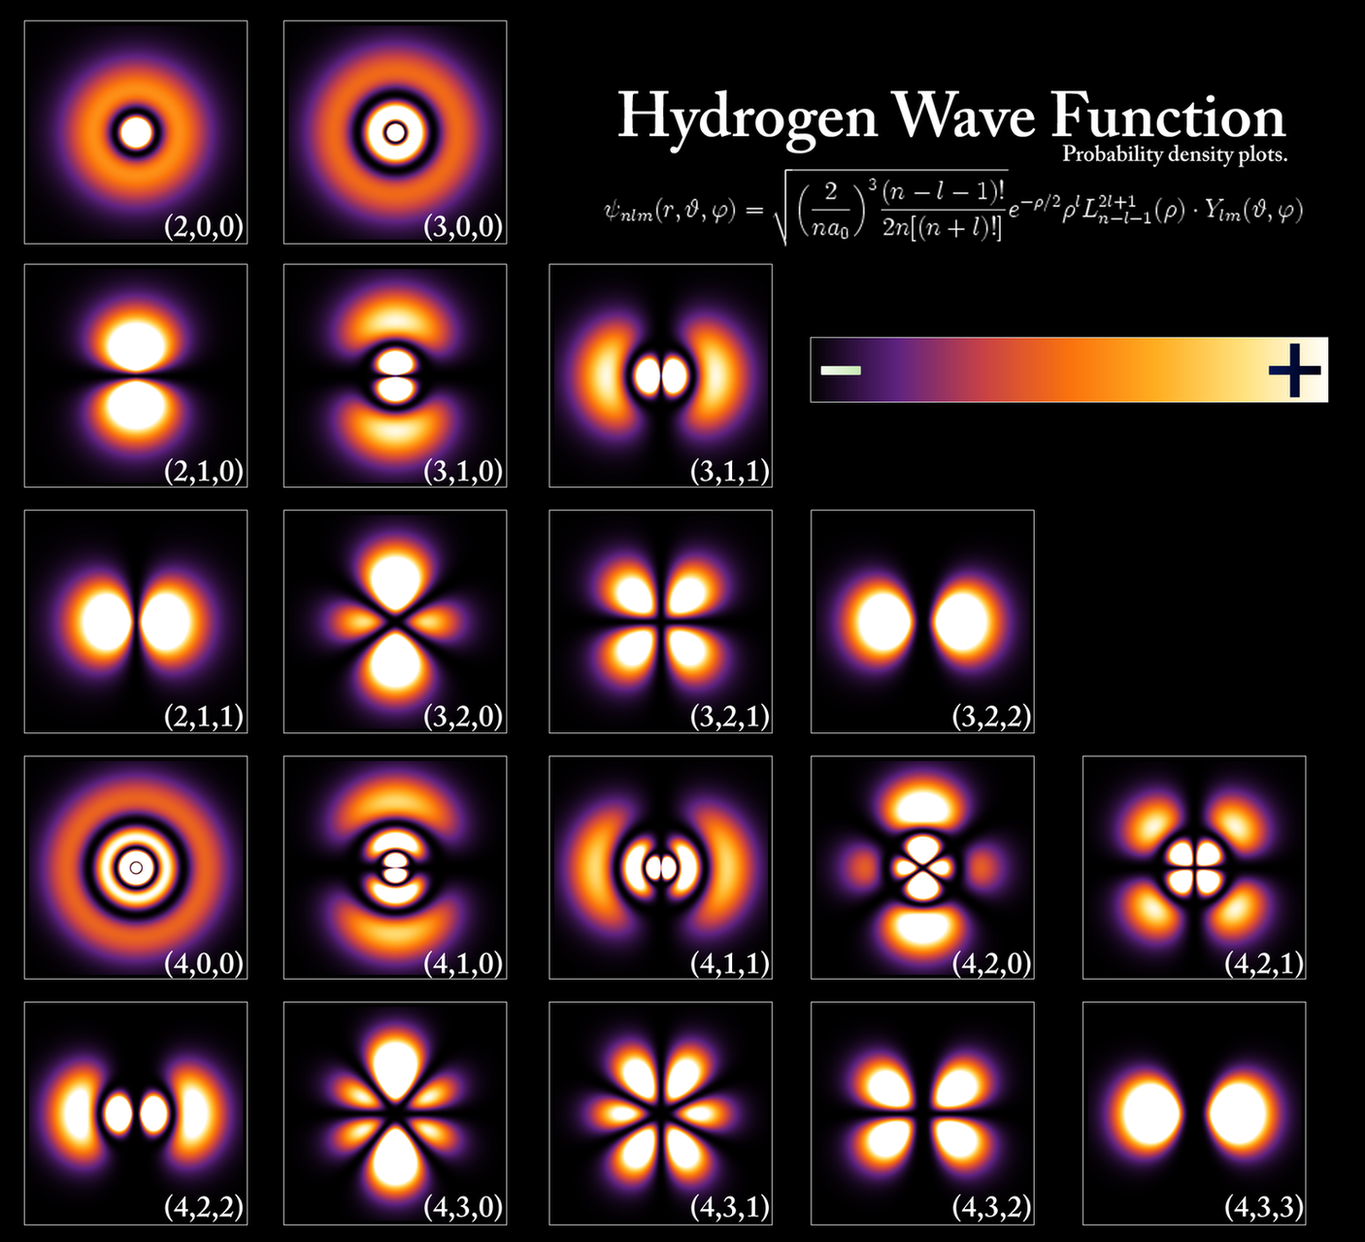
\includegraphics[width=1.\textwidth]{fig/fig4-2.png}
  \caption{Density plot of the wavefunction $\abs{\psi}^2$ for different quantum number.}
  \label{fig:4-2}
\end{figure}

Notice that the wave functions depend on all three quantum numbers, the energy in Eq.~\eqref{eq:4-44} are determined by $n$ alone.
This is a peculiarity of the Coulomb poential\footnote{For the case of infinity spherical well, the energy depend also on $l$.}.
The wave function are mutually orthogonal inherit from the spherical harmonic function in Eq.~\eqref{eq:4-21}
\begin{equation}
  \label{eq:4-63}
  \int \psi^{*}_{nlm} \psi_{n'l'm'} r^2 \sin \theta \dd  \dd \theta \dd \phi = \delta_{nn'} \delta_{ll'} \delta_{mm'},
\end{equation}
where $\delta_{n n'}$ is from the fact that they are eigenfunction of different eigenvalues from the Hamiltonian.

\subsection{The spectrum of Hydrogen}
In principle, if you put a hydrogen atom into some station state $\Psi_{nlm}$, is should stay there forever.
However if you tickle it silghtly (by collision with other atom, or by shining light on it), the electron may undergo a \textbf{transition} to some other station state --- either by absorbing energy and moving up to a higher-energy state, or by giving off energy and moving down.
In practice such perturbations are always present; transitions are constantly occurring, and the result is that a container of hydrogen gives off phonons, whose energy corresponds to the difference in energy between the initial and final states
\begin{equation}
  \label{eq:4-64}
  E_{\gamma} = E_i-E_f = -13.6 \left( \frac{1}{n_{i}^2} - \frac{1}{n_{f}^{2}} \right) .
\end{equation}

According to \textbf{Planck formula}, the energy of a photon is proportional to its frequency
\begin{equation}
  \label{eq:4-65}
  E_{\gamma}  = h \nu
\end{equation}
Meanwhile, the wavelength is given by $\lambda = \frac{c}{\nu}$, so
\begin{equation}
  \label{eq:4-66}
  \frac{1}{\lambda}= R \left( \frac{1}{n_{f}^{2}} - \frac{1}{n_{i}^{2}} \right)
\end{equation}
where
\begin{equation}
  \label{eq:4-67}
  R \equiv \frac{m}{4\pi c \hbar^{2}}  \left( \frac{e^{2}}{4 \pi \epsilon_{0}} \right)^2 = 1.097 \times 10^7 \text{m}^{-1}
\end{equation}
is known as the \textbf{Rydberg constant}.
Equation ~\eqref{eq:4-66} is the \textbf{Rydberg formula} for the spectrum of hydrogen.
This is discovered empiically in the nineteenth centry, and it was Bohr's theory to explain the result and calculate $R$ in terms of the fundamental constants of nature.

\section{Angular momentum}
For stationary state, the hydrogen atom are labeled by three quantum numbers: the principal quantum number, $n$, determines the energy of the state; for $l$ and $m$ are related to the orbital angular momentum.
In classical theory of central forces, energy and angular momentum are the fundamental conserved quantities, and it it not supersing that angular momentum plays a significant role in the quantum theory.

Classically, the angular momentum of a particle is given by
\begin{equation}
  \label{eq:4-68}
  \mathbf{L}  = \br \times \bp.
\end{equation}
The corresponding quantum operaors are obtained by the standard prescrition with $p_x \to - i\hbar \frac{\partial}{\partial x}$ and so on.

\subsection{Eigenvalues}
First the operators are not commute with each other
\begin{equation}
  \label{eq:4-69}
  \left[ L_x, L_y \right] = i\hbar L_{z} .
\end{equation}
We could cycly permutate the subindices to get the similar result for other directions.
They are the fundamantal commutation relations for angular momentum

Notice that $L_x$, $L_y$, and $L_z$ are \textit{incompatible} observables, the generalized uncertainty principle indicates that $\sigma_{L_x} \sigma_{L_y} \geq \frac{\hbar}{2} \abs{\expval{L_{z}}}$.
It would therefore be futile to look for states that are simultaneously eigenfunctions of $L_x$ and $L_y$.
On the other hand, the \textit{square of the total angular momentum}
\begin{equation}
  \label{eq:4-70}
  L^2 \equiv L_x^2 + L_y^2 + L_z^2
\end{equation}
does commute with $L_{i=x,y,z}$
\begin{equation}
  \label{eq:4-71}
  \left[ L^2, L_{i=x,y,z} \right] =0.
\end{equation}
or, in a more compact way\footnote{To prove the relation, we use the follow identity $\left[ AB,C \right] = A \left[ B,C \right] + \left[ A,C \right]B$.}
\begin{equation}
  \label{eq:4-72}
  \left[ L^2, \bL \right] =0.
\end{equation}
So $L^2$ is compatible with each component of $\bL$, and we can hope to find simultaneous eigenstates of $L^2$ and $L_z$ for example,
\begin{equation}
  \label{eq:4-73}
  L^2 f = \lambda f ~ ~ ~ \text{and} ~ ~ ~ L_z f = \mu f.
\end{equation}

Using the ladder operator technique
\begin{equation}
  \label{eq:4-74}
  L_{\pm} \equiv L_x \pm i L_{y}.
\end{equation}
The commutator with $L_z$ and $L^{2}$ are
\begin{align}
  \label{eq:4-75}
  \left[ L_z, L_{\pm} \right] &= \pm \hbar L_{\pm}, \\
  \label{eq:4-76}
  \left[ L^2, L_{\pm} \right] &=0.
\end{align}
With Eq.~\eqref{eq:4-76}, we know that if $f$ is an eigenfunction of $L^2$ and $L_z$, so also is $L_{\pm}f$.
With Eq.~\eqref{eq:4-75} and Eq.~\eqref{eq:4-73}, we have
\begin{equation}
  \label{eq:4-77}
  L_z \left( L_{\pm} f \right) = \left( L_z L_{\pm} - L_{\pm} L_z \right) f + L_{\pm} L_z f = \pm \hbar L_{\pm} f + L_{\pm} \left( \mu f \right) = \left( \mu \pm \hbar \right) \left( L_{\pm} f \right),
\end{equation}
so $L_{\pm} f$ is an eigenfunction of $L_z$ with the \textit{new} eigenvalue $\mu \pm \hbar$.

For a given value of $\lambda$, we obtain a ladder of states, with each rung spearated form its neighbors by one unit of $\hbar$ in the eigenvalue of $L_z$.
This ladder is not infinit long, one can not reach a state for which the $z$-component exceeds the total\footnote{Formally, we have $\expval{L^{2}} = \expval{L_x^2} + \expval{L_y^2} + \expval{L_z^2}$, but we also have $\expval{L_x^2} = \braket{L_x f} \geq 0$ for $x$- and $y$-direction. Then $\lambda = \expval{L_x^2} + \expval{L_y^2} + \mu^2 \geq \mu^{2}$.}.
There must exit a ``top rung'', $f_t$, such that\footnote{Actually all we can conclude is that $L_+f_t$ is not normalizable. Check the problem.}
\begin{equation}
  \label{eq:4-78}
  L_+f_t =0.
\end{equation}

Let $\hbar l$ be the eigenvalue of $L_z$ at this top rung,
\begin{equation}
  \label{eq:4-79}
  L_zf_t =\hbar l f_t; ~ ~ ~ L^2 f_t = \lambda f_t
\end{equation}
Now, with the identity
\begin{equation}
  \label{eq:4-80}
  L^2 = L_{\pm} L_{\mp} + L_z^2 \mp \hbar L_{z}
\end{equation}
we can calculate the eigenvalue
\begin{equation*}
  L^2 f_t = \left( L_- L_+ + L_z^2 + \hbar L_z \right) f_t = \left( 0 + \hbar^2l^2 +\hbar^2 l \right) f_t = \hbar^2 l \left( l+1 \right) f_t
\end{equation*}
and hence
\begin{equation}
  \label{eq:4-81}
  \lambda = \hbar^2 l \left( l+1 \right).
\end{equation}
This tell us the eigenvalue of $L^2$ in terms of the \textit{maximum eigenvalue} of $L_z$.

Meanwhile, there is also a ``bottom rung'', $f_b$, such that $L_- f_b = 0$.
Let $\hbar \bar{l}$ be the eigenvalue of $L_z$ at this bottom rung $L_z f_b = \hbar \bar{l}f_{b}$.
Using Eq.~\eqref{eq:4-80}, we have
\begin{equation}
  \label{eq:4-82}
  \lambda = \hbar^2 \bar{l} \left( \bar{l} - 1 \right).
\end{equation}
Comparing Eq.~\eqref{eq:4-81} and Eq.~\eqref{eq:4-82}, we see that $l \left( l+1 \right) = \bar{l} \left( \bar{l}-1 \right)$, so either $\bar{l} = l+1$ (which is absurd, the bottom rung is higher than the top rung) or else
\begin{equation}
  \label{eq:4-83}
  \bar{l} = -l.
\end{equation}

Appearently, from Eq.~\eqref{eq:4-83}, we known the eigenvalue of $L_z$ are $m\hbar$ where $m$ goes form $-l$ to $+l$ in $N$ integer steps.
In particular, it follows that $l=-l +N$, and hence $l= \frac{N}{2}$, so $l$ \textit{must be an integer or a half-integer}.
Then the eigenfunctions are characterized by the number $l$ and $m$
\begin{equation}
  \label{eq:4-84}
  L^2 f_l^m = \hbar^2 l \left( l+1 \right) f_l^m; ~ ~ ~ L_zf_l^m = \hbar m f_l^m
\end{equation}
where
\begin{equation}
  \label{eq:4-85}
  l = 0, \frac{1}{2}, 1, \frac{3}{2}, \ldots ; ~ ~ ~  m = -l, -l+1, \ldots, l-1, l.
\end{equation}
For a given value $l$, there are $2l+1$ different values of $m$.

Usually, peopel like to illustrate this result with the diagram Fig.~\ref{fig:4-3}.
\begin{figure}[h]
  \centering
  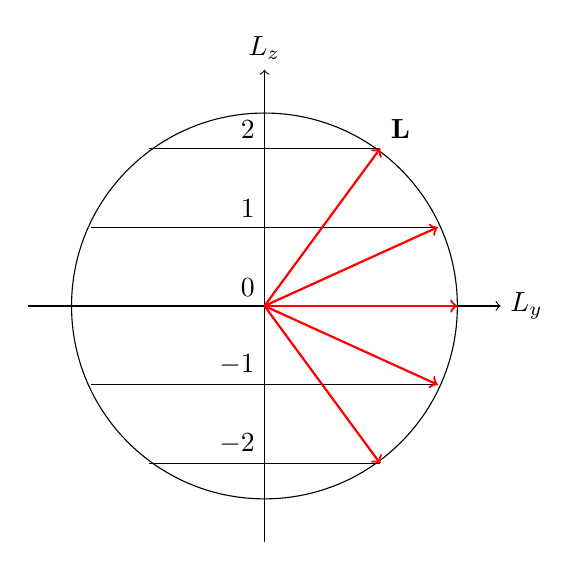
\begin{tikzpicture}
    \draw [->] (0,-3) -- (0,3);
    \draw [->] (-3,0) -- (3,0);
    \draw (0,0) circle [radius=2.45];
    \draw (-1.47,2) -- (1.47,2);
    \draw (-2.2,1) -- (2.2,1);
    \draw (-1.47,-2) -- (1.47,-2);
    \draw (-2.2,-1) -- (2.2,-1);
    \draw [thick, red, ->] (0,0) -- (1.47,2);
    \draw [thick, red, ->] (0,0) -- (2.2,1);
    \draw [thick, red, ->] (0,0) -- (2.45,0);
    \draw [thick, red, ->] (0,0) -- (1.47,-2);
    \draw [thick, red, ->] (0,0) -- (2.2,-1);
    \node [above left] at (0,2)  {$2$};
    \node [above left] at (0,1)  {$1$};
    \node [above left] at (0,0)  {$0$};
    \node [above left] at (0,-1)  {$-1$};
    \node [above left] at (0,-2) {$-2$};
    \node [above] at (0,3) {$L_z$};
    \node [right] at (3,0) {$L_y$};
    \node [above right] at (1.48, 2) {$\mathbf{L}$};
  \end{tikzpicture}
  \caption{Angular momentum startes for $l=2$.}
  \label{fig:4-3}
\end{figure}
The red arrows are supposed to represent possible angular momenta --- in units of $\hbar$ where they all have same length $\sqrt{l \left( l+1 \right)}$ and their $z$ components are allowed values of $m=-2,-1,0,1,2$.
Notice that the magnitude of the vectors is greater than the maximum $z$ component\footnote{In general, $\sqrt{l \left( l+1 \right)} > l$, except for the ``trival'' case $l=0$.}.
Evidently, you can not get the angular momentum to point perfectly along the $z$ direction.
Since to do this, you have to know all thee components simutaneously($L_x=L_y=0, L_z = \sqrt{l \left( l+1 \right)}$), and the uncertainty priciple tell us that is impossible.
It is not merely that you don't know all three components of $\mathbf{L}$; there simply aren't three components---a particle just cannot have a determinate angular momentum vector, any moer than it can simultaneously have a determinate position and moemntum.
If $L_z$ has a well-defined value, the $L_x$ and $L_y$ do not.

So, by purely algebraic means, starting with the fundamental commutation relations for angular momentum Eq.~\eqref{eq:4-69}, we have determined the eigenvalues of $L^2$ and $L_z$---without ever seeing the eigenfunctions themselves!
For the eigenfunctions, $f_l^m=Y_l^m$---the eigenfunctions of $L^2$ and $L_z$ are noting but the old sperical harmoincs function in Eq.~\eqref{eq:4-20}.
Since they are eigenfunctions of hermitian operators, $L^2$ and $L_z$, belonging to distinct eigenvalues.

\subsection{Eigenfunctions}
First, we rewrite the angular momentum in sperical coordinates, since $\mathbf{L} = \frac{\hbar}{i} \left( \mathbf{r} \times \nabla \right)$, and the gradient
\begin{equation}
  \label{eq:4-86}
  \nabla = \hat{r} \frac{\partial}{\partial r} + \hat{\theta} \frac{1}{r} \frac{\partial}{\partial \theta} + \hat{\phi} \frac{1}{r\sin\theta} \frac{\partial}{\partial \phi}
\end{equation}
meanwhile, $\mathbf{r}= r \hat{r}$, so
\begin{equation}
  \label{eq:4-87}
  \mathbf{L} = \frac{\hbar}{i} \left( \hat{\phi} \frac{\partial}{\partial \theta} - \hat{\theta} \frac{1}{\sin \theta} \frac{\partial}{\partial \phi} \right) .
\end{equation}
The unit vectors $\hat{\theta}$ and $\hat{\phi}$ can be resolved into their cartesian components due to Fig.~\ref{fig:4-1}
\begin{align}
  \label{eq:4-88}
  \hat{\theta} &= \left( \cos\theta \cos\phi \right) \hat{x} + \left( \cos\theta \sin\phi \right) \hat{y} - \left( \sin\theta \right) \hat{z} \\
  \label{eq:4-49}
  \hat{\phi} &= -\left( \sin\phi \right) \hat{x} + lr(\cos\phi) \hat{y}
\end{align}
Thus we have
\begin{align}
  \label{eq:4-90}
  L_x &= \frac{\hbar}{i} \left( -\sin\phi \frac{\partial}{\partial \theta} - \cos\phi \cot \theta \frac{\partial}{\partial \phi} \right),\\
  \label{eq:4-91}
  L_y &= \frac{\hbar}{i} \left( +\cos\phi \frac{\partial}{\partial \theta} - \sin\phi \cot \theta \frac{\partial}{\partial \phi} \right),\\
  \label{eq:4-92}
  L_z &= \frac{\hbar}{i} \frac{\partial}{\partial \phi}.
\end{align}
For descending and increasing operators
\begin{equation}
  \label{eq:4-93}
  L_{\pm} = \pm \hbar e^{\pm \phi} \left( \frac{\partial}{\partial \theta} \pm i \cot \theta \frac{\partial}{\partial \phi} \right).
\end{equation}
and $L^2$,
\begin{equation}
  \label{eq:4-94}
  L^2 = -\hbar^2 \left[ \frac{1}{\sin\theta} \frac{\partial}{\partial \theta} \left( \sin\theta \frac{\partial}{\partial \theta} \right) + \frac{1}{\sin^{2} \theta} \frac{\partial^{2}}{\partial \phi^{2}} \right] .
\end{equation}

We are now in a position to determine $f_l^m \left( \theta,\phi \right)$.
It's an eigenfunction of $L^2$, with eigenvalue $\hbar^2 l \left( l+1 \right)$.
This is precisely the angular equation, Eq.~\eqref{eq:4-9}.
And it is also an eigenfunction of $L_z$, with the eigenvalue $m\hbar$.
This is equivalent to the azimuthal equation Eq.~\eqref{eq:4-11}.
So the conclusion is the following: Spherical harmonics functions are eigenfunctions of $L^2$ and $L_z$.
When we solved the Sch\"dinger equation by separation of variables, we were inadvertently constructing simultaneous eigenfunction of the three commuting operators $H$, $L^2$, and $L_z$.

At last, there is a curious final twist to this story, for the algebraic theory of angular momentum permits $l$ to take on \textit{half-integer} values in Eq.~\eqref{eq:4-85}, whereas separation of variables yielded eigenfunctions only for \textit{integer} values in Eq.~\eqref{eq:4-17}.
n the following section, we will see the profound importance for the half-integer solutions.

\section{Spin}
In classical mechanics, a rigid object admits two kinds of angular momentum: \textbf{orbital}, associated with the motion of the center of mass, and \textbf{spin}, associated with motion about the center of mass.
For quantum mechanics, in addition to orbital angular momentum, associated with the motion of the electron around the nucleus(described by spherical harmonics in hydrogen), the electron also carries another form of angular momentum, which has nothing to do with motion in space.
The electron is a structureless point particle, and its spin angular momentum cannot be decomposed into  orbital angular momenta of constituent part.
Suffice it to say that elementary particles carry \textbf{intrinsic} angular momentum in addition to their ``extrinsic'' angular momentum.

The \textit{algebraic} theory of spin is a carbon copy of the theory of orbital angular momentum, beginning with the fundamental commutation relation
\begin{equation}
  \label{eq:4-95}
  \left[ S_i, S_j \right] = i\hbar S_k .
\end{equation}
It follows that the eigenvectors of $S^2$ and $S_z$ satisfy
\begin{equation}
  \label{eq:4-96}
  S^2 \ket{sm} = \hbar^2 s \left( s+1 \right) \ket{sm}; ~ ~ ~ S_z \ket{sm} = \hbar m \ket{sm};
\end{equation}
and
\begin{equation}
  \label{eq:4-97}
  S_{\pm} \ket{sm} = \hbar \sqrt{s \left( s+1 \right) - m \left( m \pm 1 \right)} \ket{s \left(m \pm 1 \right)} ,
\end{equation}
where $S_{\pm} \equiv S_x \pm i S_y$.
But this time the eigenvectors are not spherical harmonics(they are not functions of $\theta$ and $\phi$ at all), and there is no a \textit{priori} reason to exclude the half-integer values of $s$ and $m$
\begin{equation}
  \label{eq:4-98}
  s = 0, \frac{1}{2}, 1, \frac{3}{2}, \ldots ; ~ ~ ~  m=-s, -s+1, \ldots, s-1, s.
\end{equation}

It so happens that every elementary particle has a specific and immutable value of $s$, which we call \textbf{the spin} of the particular species: pi mesons have spin $0$; electron have spin $\frac{1}{2}$; photons have spin $1$; deltas have spin $\frac{3}{2}$; gravitions have spin  $2$; and so on.
By contrast, the orbital angular momentum quantum number $l$ can take on any integer value, and will change from one to another when the system is perturbed.
But $s$ is fixed, for any given particle, and this makes the theory of spin comparatively simple.

\subsection{Spin $\frac{1}{2}$}
By far the most important case is $s= \frac{1}{2}$, for this is the spin of the particles taht make up ordinary matter (protons, neutrons, and electrons), as well as all quarks and all leptons.
There are just two eigenstates which we call it \textbf{spin up} $\ket{ \frac{1}{2} \equiv \uparrow}$ and \textbf{spin down} $\ket{ - \frac{1}{2} \equiv \downarrow}$.
Using the basis vectors the general state of a spin-$\frac{1}{2}$ particle can be expressed as a two-element column spinor
\begin{equation}
  \label{eq:4-99}
  \chi =
  \begin{pmatrix}
    a \\
    b
  \end{pmatrix}
  =a \chi_+ + b \chi_-,
\end{equation}
with
\begin{equation}
  \label{eq:4-100}
  \chi_+ =
  \begin{pmatrix}
    1\\
    0
  \end{pmatrix}, ~ ~ ~
  \chi_- =
  \begin{pmatrix}
    0\\
    1
  \end{pmatrix}
\end{equation}
representing spin up and spin down.

Meanwhile, the spin operators become $2\times 2$ matrices.
From Eq.~\eqref{eq:4-96}, we known for $S^2$,
\begin{equation}
  \label{eq:4-101}
  S^2 \chi_{\pm}= \frac{3}{4} \hbar^2 \chi_{\pm}, ~ ~ ~
  S^2 = \frac{3}{4} \hbar^2
  \begin{pmatrix}
    1 & 0 \\
    0 & 1
  \end{pmatrix}.
\end{equation}
Similarly, for $S_z$ we have
\begin{equation}
  \label{eq:4-102}
  S_z \chi_{\pm} = \pm \frac{\hbar}{2} \chi_{\pm}, ~ ~ ~
  S_z = \frac{\hbar}{2}
  \begin{pmatrix}
    1 & 0 \\
    0 & 1
  \end{pmatrix}.
\end{equation}

Consider the properties of ladder operators, we have
\begin{equation}
  \label{eq:4-103}
  S_+ = \hbar
  \begin{pmatrix}
    0 & 1 \\
    0 & 0
  \end{pmatrix}
  , ~ ~ ~
  S_- = \hbar
  \begin{pmatrix}
    0 & 0 \\
    1 & 0
  \end{pmatrix}.
\end{equation}
Since $S_{\pm} =S_x \pm i S_y$, we have
\begin{equation}
  \label{eq:4-104}
  S_x = \frac{\hbar}{2}
  \begin{pmatrix}
    0 & 1 \\
    1 & 0
  \end{pmatrix}, ~ ~ ~
  S_y = \frac{\hbar}{2}
  \begin{pmatrix}
    0 & -i \\
    i & 0
  \end{pmatrix}.
\end{equation}
To make it tidier, we may write $\mathbf{S} = \frac{\hbar}{2} \mathbf{\sigma}$, where
\begin{equation}
  \label{eq:4-105}
  \sigma_x \equiv
  \begin{pmatrix}
    0 & 1\\
    1 & 0
  \end{pmatrix}
  , ~ ~ ~
  \sigma_y \equiv
  \begin{pmatrix}
    0 & -i \\
    i & 0
  \end{pmatrix}
  , ~ ~ ~
  \sigma_z \equiv
  \begin{pmatrix}
    1 & 0 \\
    0 & -1
  \end{pmatrix}.
\end{equation}
These are the famous \textbf{Pauli spin matrices}.
Notice that $S_x$, $S_y$, $S_z$, and $S^2$ are all hermitian.
On the other hand, $S_{\pm}$ are not hermitian.

The eigenstates of $S_z$ are
\begin{equation}
  \label{eq:4-106}
  \chi_+=
  \begin{pmatrix}
    1 \\
    0
  \end{pmatrix}
  , ~ ~ ~
  \chi_-=
  \begin{pmatrix}
    0 \\
    1
  \end{pmatrix}.
\end{equation}
If you measure $S_z$ on a particle in the geaneral state $\chi$ in Eq.~\eqref{eq:4-99}, you could get $+ \frac{\hbar}{2}$ with probabilty $\abs{a}^{2}$ and $- \frac{\hbar}{2}$ with probability $\abs{b}^{2}$.

If you measure $S_x$, then, what are the possible result and their probabilities?
First, we need to know the eigenvalues and eigenstates of $S_x$.
The characteristic equation is nothing but
\begin{equation*}
  \begin{vmatrix}
    -\lambda & \frac{\hbar}{2} \\
    \frac{\hbar}{2} & -\lambda
  \end{vmatrix}
  = 0  \to \lambda = \pm \frac{\hbar}{2}.
\end{equation*}
The normalized eigenstates of $S_x$ are
\begin{equation}
  \label{eq:4-107}
  \chi_+^x =
  \begin{pmatrix}
    \frac{1}{\sqrt{2}}\\
    \frac{1}{\sqrt{2}}
  \end{pmatrix}, ~ ~ ~
  \chi_-^x =
  \begin{pmatrix}
    \frac{1}{\sqrt{2}}\\
    - \frac{1}{\sqrt{2}}
  \end{pmatrix}.
\end{equation}
The generic spinor Eq.~\eqref{eq:4-99} can be expressed as a linear combination.

\subsection{Electron in a magnetic field: Basic}
A spinning charged particle constitutes a magnetic dipole.
Its \textbf{magnetic dipole momentum} $\mu$ is proportional to its spin angular momentum
\begin{equation}
  \label{eq:4-108}
 \boldsymbol{\mu} = \gamma \mathbf{S}
\end{equation}
the proportionality constant $\gamma$ is called the \textbf{gyromagnetic ratio}.
With a magnetic field $\mathbf{B}$, it experiences a torque, $\boldsymbol{\mu} \times \mathbf{B}$, which tends to line it up parallel to the field.
The energy associated with this torque is
\begin{equation}
  \label{eq:4-109}
 H = - \boldsymbol{\mu} \cdot \mathbf{B},
\end{equation}
so the Hamiltonian of a spinning charged particle, at rest\footnote{If a particle is allowed to move, there will be kinetic energy and Lorentz force, which is not derivable from a potential energy function and hence does not fit the Schr\"odinger equation as we formulated so far.} in a magnetic field $\mathbf{B}$ is
\begin{equation}
  \label{eq:4-110}
  H = - \gamma \mathbf{B} \cdot \mathbf{S}.
\end{equation}

\subsection{Larmor precession}
Imagine a particle of spin $\frac{1}{2}$ at rest in a uniform magnetic field, which points in the $z$-direction
\begin{equation}
  \label{eq:4-111}
 \mathbf{B} = B_0 \hat{z}.
\end{equation}
The Hamiltonian in matrix form is
\begin{equation}
  \label{eq:4-112}
 H = - \gamma B_0 S_z = - \frac{\gamma B_0 \hbar}{2}
 \begin{pmatrix}
   1 & 0 \\
   0 & 1
 \end{pmatrix}.
\end{equation}
The eigenstate of this $H$ are the same as those of $S_z$ in Eq.~\eqref{eq:4-106} with energy $E_{\pm} = \mp \frac{\gamma B_0 \hbar}{2}$.

Since the Hamiltonian is time-independent, the general solution the the time-dependent Schr\"odinger equation, $i\hbar \frac{\partial \chi }{\partial t} = H \chi$, can be expressed in terms of stationary states
\begin{equation*}
  \chi \left( t \right) =
  \begin{pmatrix}
    \cos \left( \frac{\alpha}{2} \right) e^{i\gamma B_0 t/2} \\
    \sin \left( \frac{\alpha}{2} \right)  e^{-i \gamma B_0 t/2}
  \end{pmatrix}.
\end{equation*}
The constants $\cos \left( \frac{\alpha}{2} \right)$ and $\sin \left( \frac{\alpha}{2} \right)$ are determined by the initial condition and the physical importance of the phase angle $\alpha$ will discussed later.

One can calculate the expectation value of $\mathbf{S}$ as a function of time
\begin{align}
  \label{eq:4-113}
 \expval{S_x} &= \chi \left( t \right)^{\dagger} S_x \chi \left( t \right) = \frac{\hbar}{2} \sin \alpha \cos \left( \gamma B_0 t \right) \\
  \label{eq:4-114}
 \expval{S_y} &= \chi \left( t \right)^{\dagger} S_y \chi \left( t \right) = \frac{\hbar}{2} \sin \alpha \sin \left( \gamma B_0 t \right) \\
  \label{eq:4-115}
 \expval{S_z} &= \chi \left( t \right)^{\dagger} S_z \chi \left( t \right) = \frac{\hbar}{2} \cos \alpha
\end{align}
Evidently $\expval{\mathbf{S}}$ is tilted at a constant angle $\alpha$ to the $z$-axis, and precesses about the field at the \textbf{Larmor frequency}
\begin{equation}
  \label{eq:4-116}
 \omega = \gamma B_0,
\end{equation}
just as it would classically.
This is because the Ehrenfest's theorem guarantees that $\expval{\mathbf{S}}$ evolves according to the classical laws.

For example, the \textbf{Stern-Gerlach experiment} is an application of this effect as shwon in Fig.~\ref{fig:4-4}.
In an \textit{inhomogeneous} magnetic field, there is not only a \textit{torque}, but also a force on a magnetic dipole\footnote{We assume a neutral particle to avoid the Lorentz force and heavy so we can construct localized wave packets and treat the motion in terms of classical particle trajectories. In practice, the Stern-Gerlach experiment does not work, for example, with a beam of free electrons.}
\begin{equation}
  \label{eq:4-117}
 \mathbf{F} = \nabla \left( \boldsymbol{\mu} \cdot \mathbf{B} \right) .
\end{equation}
This force can be used to separate out particles with a particular spin orientation.
Imagine a beam of relatively heavy neutral atom which pass through a region of inhomogeneous magnetic field
\begin{equation}
  \label{eq:4-118}
 \mathbf{B} \left( x,y,z \right) = -\alpha x \hat{x} + \left( B_0 + \alpha z \right) \hat{z}
\end{equation}
where $B_0$ is a strong uniform field and the constant $\alpha$ describes a small deviation from homogeneity\footnote{We can not have something only with $z$ component in this case, since it breaks the electromagnetic law $\nabla \cdot \mathbf{B} = 0$.}.

\begin{figure}[t]
  \centering
  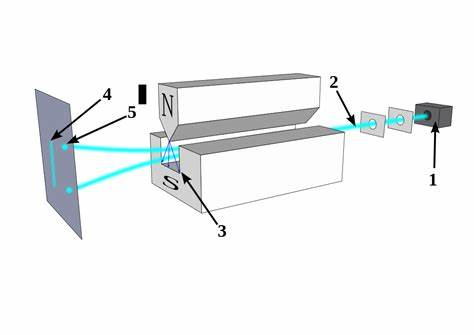
\includegraphics[width=0.75\textwidth]{fig/fig4-3.png}
  \label{fig:4-4}
  \caption{The setup of Stern-Gerlach experiment. (1) source; (2) hole; (3) inhomogeneous magnetic field; (4) the classical expectation and (5) the observation.}
\end{figure}

The corresponding force on the atom is
\begin{equation*}
  \mathbf{F} = \gamma \alpha \left( -S_x \hat{x} + S_z \hat{z} \right) .
\end{equation*}
However, as Eq.~\eqref{eq:4-113} suggested, due to the Larmor precession about $B_0$, $S_x$ oscillates rapidly and averages to zero.
The \textit{net} force is purely in the $z$ direction
\begin{equation}
  \label{eq:4-119}
 F_z = \gamma \alpha S_z
\end{equation}
and the beam is deflected up or down, in proportion to the $z$ component of the spin angular momentum.

In the more \textit{quantum} argument, we examine the process from the perspective of a reference frame that moves along with the beam.
In this frame the Hamiltonian starts out zero, turns on for a time $T$ and then turn off again
\begin{equation}
  \label{eq:4-120}
  H \left( t \right) =
  \begin{cases}
    0,~ ~ ~ &\text{for $t<0$} \\
    -\gamma \left( B_0 + \alpha a \right) S_z, ~ ~ ~ &\text{for $0\leq t \leq T$}\\
    0,~ ~ ~  &\text{for $t>T$}
  \end{cases},
\end{equation}
where we have ignore the $x$ component contribution from $\mathbf{B}$ for the same reason discussed before.
Suppose the atom has spin $\frac{1}{2}$ and starts out in the state
\begin{equation*}
\chi(t) = a \chi_+ + b \chi_- ~ ~ ~ \text{for $t\leq 0$}.
\end{equation*}
In the magnetic filed region where the non-zero Hamiltonian acts, we have
\begin{equation*}
\chi \left( t \right) = a \chi_+ e^{-i E_+ t/hbar} + b \chi_- e^{-iE_-t/\hbar} ~ ~ ~ \text{for $0\leq t \leq T$},
\end{equation*}
where
\begin{equation}
  \label{eq:4-121}
  E_{\pm} = \mp \gamma \left( B_0 +\alpha z \right) \frac{\hbar}{2}
\end{equation}
and hence it emerges in the state
\begin{equation}
  \label{eq:4-122}
  \chi \left( t \right) = \left( a e^{i\gamma T B_0/2} \chi_+ \right) e^{i \left( \alpha \gamma T/2 \right)z} + \left( b e^{-i\gamma T B_0/2} \chi_- \right) e^{-i \left( \alpha \gamma T/2 \right)z}.
\end{equation}
The two terms now carry \textit{momentum} in the $z$ direction
\begin{equation}
  \label{eq:4-123}
 p_z = \pm \frac{\alpha \gamma T \hbar}{2}.
\end{equation}
Thus $\chi_+$ will moves in the plus-$z$ direction and opposite for $\chi_-$ state.

\subsection{Addition of angular momenta}
Suppose now that we have two spin-$\frac{1}{2}$ particles---for example, the electron and the proton in the ground state of hydrogen.
Each can have spin up or spin down, so there are four possibilities in all\footnote{We consider the ground state, so there  will not any orbital angular momentum to worry about.}
\begin{equation}
  \label{eq:4-124}
 \ket{\uparrow \uparrow}, ~ \ket{\uparrow \downarrow},~ \ket{\downarrow \uparrow}, ~ \ket{\downarrow \downarrow},
\end{equation}
where the first arrow refer to the electron and the second to the proton.
We want to know what is the total angular momentum of the atom $\mathbf{S} \equiv \mathbf{S}_1 + \mathbf{S}_{2}$.
Since each of these four composite states in Eq.~\eqref{eq:4-124}, is an eigenstate of $S_z$, we have
\begin{equation*}
  S_z\ket{\chi_1 \chi_2} = \left( S_1 + S_2 \right) \ket{\chi_1 \chi_2} = \hbar \left( m_1 + m_2 \right) \ket{\chi_1 \chi_2}
\end{equation*}
So $m$ is just $m_1+m_2$:
\begin{align*}
  m &=1 ~ ~ ~ \ket{\uparrow \uparrow}\\
  m &=0 ~ ~ ~ \ket{\uparrow \downarrow}\\
  m &=0 ~ ~ ~ \ket{\downarrow \uparrow}\\
  m &=-1 ~ ~ ~ \ket{\downarrow \downarrow}.
\end{align*}

At first glance, this does not look right: $m$ is suppose to advance in integer steps from $-s$ to $+s$ where $s=1$ in our case.
However, there is an ``extra'' state with $m=0$.
One way to untangle this problem is to apply the lowering operator to the state $\ket{\uparrow \uparrow}$
\begin{equation*}
  S_- \ket{\uparrow \uparrow} = \hbar \left( \ket{\downarrow \uparrow} + \ket{\uparrow \downarrow} \right).
\end{equation*}
Evidently, in the notation of $\ket{sm}$, the three stats with $s=1$ are
\begin{equation}
  \label{eq:4-125}
  s = 1 ~ \text{(triplet state)} ~ \to
  \begin{cases}
    \ket{11} &= \ket{\uparrow \uparrow} \\
    \ket{10} &= \frac{1}{\sqrt{2}} \left( \ket{\uparrow \downarrow} + \ket{\downarrow \uparrow} \right)\\
    \ket{1-1} &= \ket{\downarrow \downarrow}
  \end{cases}.
\end{equation}
This is called the \textbf{triplet} combination.
Meanwhile, the orthogonal state with $m=0$ carries $s=0$
\begin{equation}
  \label{eq:4-126}
  s = 0 ~ \text{(singlet state)} ~ \to \ket{00} = \frac{1}{\sqrt{2}} \left( \ket{\uparrow\downarrow} - \ket{\downarrow \uparrow} \right).
\end{equation}

We found that the combination of two spin-$\frac{1}{2}$ particles can carry a total spin of $1$ and $0$, depending on whether they occupy the triplet or the single configuration.
To verify this, we will prove that the triplet states are eigenvectors of $S^2$ with eigenvalue $\hbar^{2} s \left( s+1 \right) = 2\hbar^{2}$ and single is for eigenvalue $0$.
Now,
\begin{equation}
  \label{eq:4-127}
 S^2 = \left( \mathbf{S}_1 + \mathbf{S}_2 \right) \cdot \left( \mathbf{S}_1 + \mathbf{S}_2 \right) = S_1^2 + S_2^2 + 2 \mathbf{S}_1 \cdot \mathbf{S}_2.
\end{equation}
Using Eq.~\eqref{eq:4-102} and Eq.~\eqref{eq:4-104}, we have
\begin{align*}
  & \mathbf{S}_1 \cdot \mathbf{S}_2 \ket{\uparrow \downarrow} \\
  =& \left( S_{x1}S_{x2} + S_{y1}S_{y2} + S_{z1}S_{z2} \right) \ket{\uparrow\downarrow}\\
  =& \frac{\hbar^{2}}{4} \left( 2\ket{\downarrow\uparrow} - \ket{\uparrow\downarrow} \right).
\end{align*}
Similarly,
\begin{equation*}
   \mathbf{S}_1 \cdot \mathbf{S}_2 \ket{\downarrow \uparrow}  =  \frac{\hbar^{2}}{4} \left( 2 \ket{\uparrow \downarrow} - \ket{\downarrow\uparrow} \right).
\end{equation*}
Then returning to Eq.~\eqref{eq:4-125}, we have
\begin{equation}
  \label{eq:4-128}
  S^2 \ket{10} = \left( \frac{3\hbar^{2}}{4} + \frac{3\hbar^{2}}{4} + 2 \frac{\hbar^{2}}{4} \right) \ket{10} = 2\hbar^2 \ket{10},
\end{equation}
so $\ket{10}$ is indeed an eigenstate of $s^2$ with eigenvalue $2\hbar^{2}$.
We can did the similar calculation for $\ket{00}$ and we have $S^2 \ket{00}= 0 \ket{00}$.

This is the simplest example of a larger problem: If you combine spin $s_1$ with spin $s_2$, the total spins $s$ you can get is
\begin{equation}
  \label{eq:4-129}
 s = \left( s_1 + s_2 \right), \left( s_1+s_2-1 \right), \ldots, \abs{s_1-s_2},
\end{equation}
where they are in integer steps.
For example, if you package together a particle of spin $\frac{3}{2}$ with a particle of spin $2$, you could get a total spin of $\frac{7}{2}$, $\frac{5}{2}$, $\frac{3}{2}$, or $\frac{1}{2}$, depending on the configuration.
Another example, if a hydrogen atom is in the state $\psi_{nlm}$, the net angular momentum of the electron is $l+ \frac{1}{2}$ or $l - \frac{1}{2}$;
if you now throw in a \textit{proton}, the atom's total angular momentum quantum number is $l+1$, $l$, or $l-1$.

The combined state $\ket{sm}$ with total spin $s$ ans $z$-component $m$ will be some linear combination of the composite states $\ket{s_1 m_1}\ket{s_2 m_2}$:
\begin{equation}
  \label{eq:4-130}
 \ket{sm}  = \sum_{m_1+m_2=m} C_{m_1m_2m}^{s_1s_2s} \ket{s_1 m_1} \ket{s_2 m_2}.
\end{equation}
The constants $C_{m_1m_2m}^{s_1s_2s}$ are called \textbf{Clebsch-Gordan coefficients}
The simplest case are listed in Fig.~\ref{fig:4-5}.
\begin{figure}[t]
  \centering
  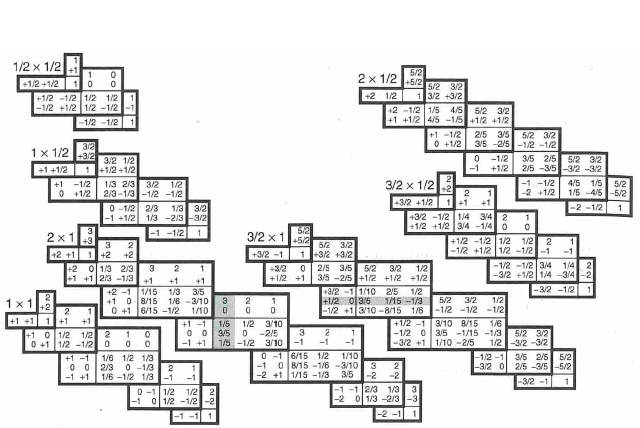
\includegraphics[width=0.95\textwidth]{fig/fig4-4.png}
  \label{fig:4-5}
  \caption{Clebsch-Gordan coefficients. A square root sign is understood for every entry; the minus sign, if present, goes outside the radical.}
\end{figure}
For example, the shaded column of $2\times 1$ table tell us that
\begin{equation*}
\ket{30} = \frac{1}{\sqrt{5}}\ket{21}\ket{1-1} + \sqrt{\frac{3}{5}}\ket{20}\ket{10} + \frac{1}{\sqrt{5}}\ket{2-1}\ket{11}.
\end{equation*}
In particular, if two particles (of spin $2$ and spin $1$) are at rest in a box, and the total spin is $3$, and its $z$ component is $0$ (where $\ket{30}$), then a measurement of $S_z^1$ could return the value $\hbar$ (with probability $\frac{1}{5}$), or $0$ (with probability $\frac{3}{5}$), or $-\hbar$ (with probability $\frac{1}{5}$).

These tables also work the other way around
\begin{equation}
  \label{eq:4-131}
 \ket{s_1 m_1} \ket{s_2 m_2} = \sum_s C_{m_1m_2m}^{s_1s_2s} \ket{sm}.
\end{equation}
For example, the shaded row in the $\frac{3}{2}\times 1$ table tells us that
\begin{equation*}
  \ket{\frac{3}{2} \frac{1}{2}} \ket{10} = \sqrt{\frac{3}{5}} \ket{\frac{5}{2} \frac{1}{2}} + \sqrt{\frac{1}{15}} \ket{\frac{3}{2} \frac{1}{2}} - \sqrt{\frac{1}{3}} \ket{\frac{1}{2} \frac{1}{2}}
\end{equation*}
If you put particles of spin $\frac{3}{2}$ and spin $1$ in the box, and you know that the first has $m_1= \frac{1}{2}$ and the second has $m_2=0$, and you measure the total spin, $s$, you could get $\frac{5}{2}$ (with probability $\frac{3}{5}$), or $\frac{3}{2}$ (with probability $\frac{1}{15}$), or $\frac{1}{2}$ (with probability $\frac{1}{3}$).

In a mathematical sense this is all applied \textbf{group theory}---what we are talking about is the decomposition of the direct product of two irreducible representations of the rotation group into a direct sum of irreducible representations.










%%% Local Variables:
%%% mode: latex
%%% TeX-master: "main"
%%% End:

\chapter{Homogeneous Electron Gas}

\section{Exchange and Correlation}\label{s5.1}
The homogeneous electron gas is describe by the Hamiltonian
\begin{eqnarray}
    H &=& \sum_{\bp\sigma} \varepsilon_\bp C^\dagger_{\bp\sigma} C_{\bp\sigma} + \frac{1}{2V} \sum_{\bk\bk'\sigma\sigma'} \sum_{\bq\neq 0} v_q C^\dagger_{\bk+\bq \sigma} C^\dagger_{\bk'-\bq \sigma'} C_{\bk'\sigma'} C_{\bk\sigma} \label{5.1} \\
\varepsilon_p &=& \frac{p^2}{2m} \nonumber \\
v_q &=& \frac{4\pi e^2}{q^2} \label{5.2}
\end{eqnarray}
which was derived in \eqref{1.164}.
The free electrons mutually interact by Coulomb's law.
This $N_e$ electrons in a volume $V$ with the average density $n_0 = \frac{N_e}{V}$.
A positive charge of density $n_0$ is spread uniformly through the volume make the system charge neutrality.
The homogeneous electron gas is also called the \textbf{jellium model} of a solid.

The parameter $r_s$ is universally used to describe the density of an electro gas,
\begin{equation}
    \frac{4\pi n_0 a_0^3}{3} r_s^3 =1 \label{5.3}
\end{equation}
where $a_0$ is the Bohr radius.
$r_s$ is small for high-density electron gas and it is large for a low-density gas.
The density may related to the Fermi vector,
\begin{equation}
    n_0 = 2 \int \frac{d^3 p}{(2\pi)^3} \eta_p = \frac{1}{\pi^2} \int_0^{k_F} p^2 dp = \frac{k_F^3}{3\pi^2}     \label{5.4}
\end{equation}
so the Fermi wave vector and energy are related to $r_s$,
\begin{eqnarray}
    k_F a_0 &=& \frac{1.9192}{r_s} \nonumber \\
    E_F &=& \frac{3.6832}{r_s^2}  E_{ry}, ~ ~ ~ E_{ry}=13.60 eV \label{5.5}
\end{eqnarray}
The plasma frequency is
\begin{equation}
    \hbar \omega_p = \hbar \sqrt{ \frac{4\pi e^2 n_0}{m}  }     \label{5.6}
\end{equation}
In homogeneous electron gas, the average kinetic energy of the electrons is going to be proportional to $\langle E_F \rangle \sim k_F^2$.
Which by dimension analysis, we have $\langle E_F \rangle\propto 1/r_s^2$.
For the Coulomb energy $\langle v_p \rangle \propto 1/r_s$.
When the electron gas is sufficiently hight, $r_s$ is small, the kinetic energy term will be larger than the potential energy term, which means electrons behaves like the free particles.

\subsection{Kinetic energy}
The first energy term is kinetic energy.
The contribution to the ground state energy is obtained by summing over all particles in the ground state
\begin{eqnarray}
    E &=& \sum_{\bp \sigma} \varepsilon_p n_p = 2 V \int \frac{d^3 p}{(2\pi)^3} \frac{p^2}{2m} \eta_p = \left( \frac{N_e}{n_0} \right) \frac{1}{2\pi^2 m} \int_0^{k_F} p^4 dp \nonumber \\
&=& \frac{3}{5} \frac{\hbar^2 k_F^2}{2m} N_e = \frac{3}{5} E_F N_e = \frac{2.2099}{r_s^2} E_{ry} N_e    \label{5.8}
\end{eqnarray}
The average kinetic energy is $ \frac{3}{5} E_F$, which is given in terms of $r_s$.

\subsection{Hartee}
All the remaining terms in the energy come from the Coulomb interaction between the particles.
\textit{The first term which occurs is the Coulomb interaction between the electrons and the uniform positive background}, which is called the \textbf{Hartee interaction}.
In the model of the homogeneous electron gas, the time-averaged electron density is uniform throughout the system, as is the positive background.
These equal and opposite charge cancel each other, and Hartree energy is zero.
The energy is
\begin{equation}
    N_e E_0 = \frac{e^2}{2} \int \frac{d^3 r_1 d^3 r_2}{\abs{\br_1 - \br_2}} \left[ \rho_e(\br_1) - \rho_i(\br_1) \right] \left[ \rho_e(\br_2) - \rho_i(\br_2) \right]  \label{5.9}
\end{equation}
but the ion and electron are $\rho_e = \rho_i = n_0$, then the contribution is zero.
This fact has already been used in \eqref{5.1} by omission of the $\bq=0$ term from the Coulomb interaction.
The $\bq=0$ term is the direct Coulomb interaction among the electrons, and it is omitted because it is canceled by the direct interaction with the positive background.

\subsection{Exchange}
The Coulomb interaction in \eqref{5.1} provide other energy contributions in addition to the direct term.
For Hartee term the corresponding $H$ is given
\begin{equation}
    \sum_{\bk \bk' \sigma \sigma'} \langle C^\dagger_{\bk+\bq,\sigma} C^\dagger_{\bk'-\bq,\sigma'} C_{\bk',\sigma'} C_{\bk,\sigma} \rangle \approx \delta_{\bq = 0} \sum_{\bk\sigma} \langle C^\dagger_{\bk,\sigma} C_{\bk,\sigma} \rangle \sum_{\bk'\sigma'} \langle C^\dagger_{\bk',\sigma'} C_{\bk',\sigma'} \rangle
\end{equation}
Another way to pair the same operator gives
\begin{equation}
    \approx - \sum_{\bk\bk'\sigma\sigma'} \langle C^\dagger_{\bk+\bq,\sigma} C_{\bk',\sigma'} \rangle \langle C^\dagger_{\bk'-\bq,\sigma'} C_{\bk,\sigma'} \rangle = - \sum_{\bk\sigma} n_{\bk+\bq} n_\bk
\end{equation}
This require that $\sigma' =\sigma$ and $\bk' = \bk + \bq$.
This term is called \textbf{exchange energy (Fock energy)}.
\textit{Retaining both terms is called Hartree-Fock.}
The exchange term was derived in \eqref{2.138}, it gives a contribution to the energy of an individual electron, as well as a contribution to the ground state energy of the collection of electrons. \textbf{For per electron},
\begin{equation}
    \Sigma_x(k) = - \frac{1}{V} \sum_\bq v_q n_{\bk+\bq}    \label{5.11}
\end{equation}
\begin{equation}
    E_{gx} = - \sum_{\bk\bq\sigma} \frac{v_q}{2V}   n_{\bk+\bq} n_\bk =\frac{1}{2N_e} \sum_{\bk\sigma} n_\bk \Sigma_x(k)  \label{5.12}
\end{equation}
The self-energy $\Sigma_x(k)$ depends only on the magnitude of the wave vector $k$ of the particle and gives
\begin{eqnarray}
    \Sigma_x(k) &=& - \int \frac{d^3 p}{(2\pi)^3} \frac{4\pi e^2}{\abs{\bp -\bk}^2} n_p \nonumber \\
    &=& - \frac{e^2}{\pi}  \int_0^{k_F} p^2 dp \int_{-1}^{1} \frac{d \cos\theta}{k^2+p^2 -2pk\cos\theta} \nonumber \\
    &=& - \frac{e^2 k_F}{\pi}  \left( 1+ \frac{1-y^2}{2y} \ln \abs{\frac{1+y}{1-y}}  \right) \label{5.16} \\
    y &=& \frac{k}{k_F} \label{5.17}
\end{eqnarray}

A particle at the Fermi energy $k=k_F$ has
\begin{equation}
    \Sigma_x (k_F) = - \frac{e^2 k_F}{\pi} \label{5.18}
\end{equation}
It is convenient to write
\begin{eqnarray}
    \Sigma_x(k) &=& \frac{e^2 k_F}{\pi} S(y)    \label{5.19} \\
    S(y) &=& - \left( 1+ \frac{1-y^2}{2y} \ln \abs{ \frac{1+y}{1-y} } \right)   \label{5.20}
\end{eqnarray}
where $S(y)$ is a function which gives the wave vector dependence of the exchange energy.
\begin{figure}[ht]
    \centering
    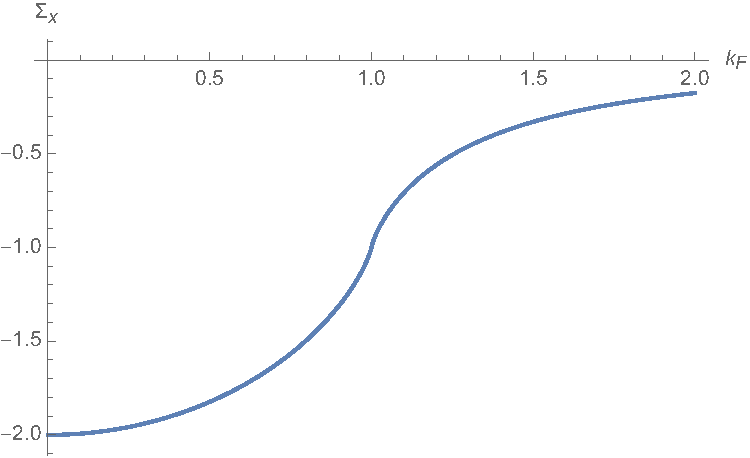
\includegraphics[width=0.4\linewidth]{./fig/fig5_1.pdf}
    \caption{Exchange energy.}%
    \label{fig:5.1}
\end{figure}
The behaviour of the function is in shown in Figure~\ref{fig:5.1}.

The derivative has a logarithmic divergence as $y\to 1$. This fact is interesting because it predicts that the effective mass is zero.
The effective mass of a particle defined in \eqref{3.160}.
Since the exchange self-energy is not frequency dependent, the effective mass is
\begin{equation}
    \left( \frac{m}{m^*} \right) = 1+ \partial_{\varepsilon_k} \Sigma_x(k) = \frac{e^2 m}{2\pi k_F } \frac{1}{y^2} \left( \frac{1+y^2}{y} \ln \abs{ \frac{1+y}{1-y} }-1  \right) \label{5.24}
\end{equation}
which diverges at Fermi energy $y\to 1$.
If the inverse effective mass really diverged at the Fermi surface, it would have several observable consequences.
The electron gas would be unstable at low temperatures, and the specific heat would diverge.
Further terms in the perturbation theory produces another divergence in the effective mass which exactly cancels the one due to exchange.
The effective mass and specific heat are not divergent.

The exchange energy contribution to the ground state energy is obtained from \eqref{5.12}.
Summing over spin gives an expression
\begin{eqnarray}
    E_{gx} &=& \frac{1}{N_e} \sum_\bk n_\bk \Sigma_x(k) = \frac{1}{n_0} \int \frac{d^3k}{(2\pi)^3} n_k \Sigma_x(k) \nonumber \\
    &=& - \frac{3}{4} \frac{e^2 k_F}{\pi} \label{5.25}
\end{eqnarray}
The average exchange energy per electron is $ \frac{3}{2} $ of the value ate the Fermi energy.
In therms of the parameter $r_s$, the total ground state exchange energy per electron is
\begin{equation}
    E_{gx} = - \frac{3}{2\pi} (k_F a_0) \left( \frac{e^2}{2a_0} \right) = - \frac{0.9163}{r_s} \label{5.26}
\end{equation}

So far two terms have been found for the energy of the particle,
\begin{equation}
    E(k) = \frac{\hbar^2 k^2}{2m} + \Sigma_x(k) + \dots \label{5.27}
\end{equation}
The corresponding two terms for the ground state energy per particle are,
\begin{equation}
    E_g = \frac{2.2099}{r_s^2} - \frac{0.9163}{r_s} + \dots \label{5.28}
\end{equation}
The ground state energy has the appearance of a power series, in increasing powers of $r_s$.
Although it is usually unsafe to extrapolate from just two terms, in fact $E_g$ is a series in $r_s$.
The next term will be of order $O(r_s^0)$.
The zeroth power could be interpreted as either a constant or as $\ln(r_s)$.
The series have the form
\begin{equation}
    E_g =  \frac{2.2099}{r_s^2} - \frac{0.9163}{r_s} -0.094 + 0.0622\ln(r_s) + \dots \label{5.29}
\end{equation}

The above energy terms comprise the Hartree-Fock theory.
It is defined to be the kinetic energy, the Hartree energy which is zero, and the exchange energy.
The total ground state energy per particle is written with correlation energy,
\begin{equation}
    E_g = \frac{2.2099}{r_s^2} - \frac{0.9163}{r_s} +E_c \label{5.30}
\end{equation}
where the correlation energy $E_c$ needs to be determined.
The result
\begin{equation}
    E_c = -0.094 + 0.0622\ln(r_s) + O(r_s) \label{5.31}
\end{equation}
is convergence when $r_s \leq 1$.

\subsection{Seitz's Theorem}
The theorem of Seitz relates the ground state energy to the chemical potential.
The chemical potential is defined as the energy it takes to add or remove an electron from the material.
It is the energy which divides the empty from the occupied states at zero temperature.
Of course, it is just the Fermi energy of the metal.
The chemical potential is the energy of an electron of momentum $k_F$
\begin{equation}
    \mu = \frac{\hbar^2 k_F^2}{2m} + \Sigma_x (k_F) + \Re \Sigma_c(k_f,0) \label{5.33}
\end{equation}
where $ik_n= 0$ is the chemical potential.
The chemical potential $\mu$ is only a function of the electron $n_0$. The theorem of Seitz is
\begin{equation}
    \mu (n_0)  = \frac{d}{d n_0}  \left[ n_0 E_g(n_0) \right] = E_g + n_0 \frac{d E_g}{d n_0} \label{5.34}
\end{equation}
The proof, by definition of chemical potential
\begin{equation}
    \mu = E_T(N_e+1) - E_T(N_e)     \label{5.35}
\end{equation}
The total energy for $N_e$ particle system is $E_T = N_e E_g$ for a fixed volume since the $E_g$ is the function of density,
\begin{eqnarray}
    E_T(N_e+1) &=& (N_e+1) E_g(n_0 + 1/V) = (N_e+1) \left( E_g(n_0) + \frac{1}{V} \frac{d E_g}{d n_0} \right) \nonumber \\
    &=& N_e E_g + E_g(n_0) + n_0 \frac{dE_g}{n_0}  + O( \frac{1}{V} )   \label{5.36}
\end{eqnarray}
In proving the theorem, the volume $V$ is kept fixed, as is the amount of positive charge.
The $N_e+1$ particle system has a slight charge imbalance, but it is negligible to the contribution of energy.
Considering a body of average dimension $L$ is uniformly charged with on unit of charge, the Coulomb energy is of order $e^2/L$.
This contribution is negligible when $L$ is large.

The chemical potential is the negative of the work function.
It is the energy required to remove an electron form the solid and take it to infinity with zero kinetic energy.
However, there is a surface correction to the work function, but not to volume part of the ground state energy per particle.
\begin{equation}
    E_T = N_e E_g + A E_S   \label{5.37}
\end{equation}
where $A$ is the total surface area and $E_S$ is the energy per unit surface area.
For macroscopic bodies, $E_g$ does not depend on the surface area.
However, $\mu$ does have a term which depends on the surface--actually on the surface dipole layer, $\mu = \mu_B + \Delta \mu$.
The theorem of Seitz actually just works on $\mu_B$.
In Hartree-Fock approximation the chemical potential gives for the bulk contribution,
\begin{equation}
    \mu_{B,HF} = \frac{d}{dn_0} \left( n_0 E_{g,HF} \right) = E_F - \frac{e^2 k_F}{\pi}     \label{5.39}
\end{equation}

\subsection{$\Sigma^{2a}$}
The exchange energy calculated involve one Coulomb line.
The correlation energy is the sum of all contribution with two or more Coulomb lines.
There are three diagrams with two Coulomb line.
\begin{figure}[ht]
    \centering
    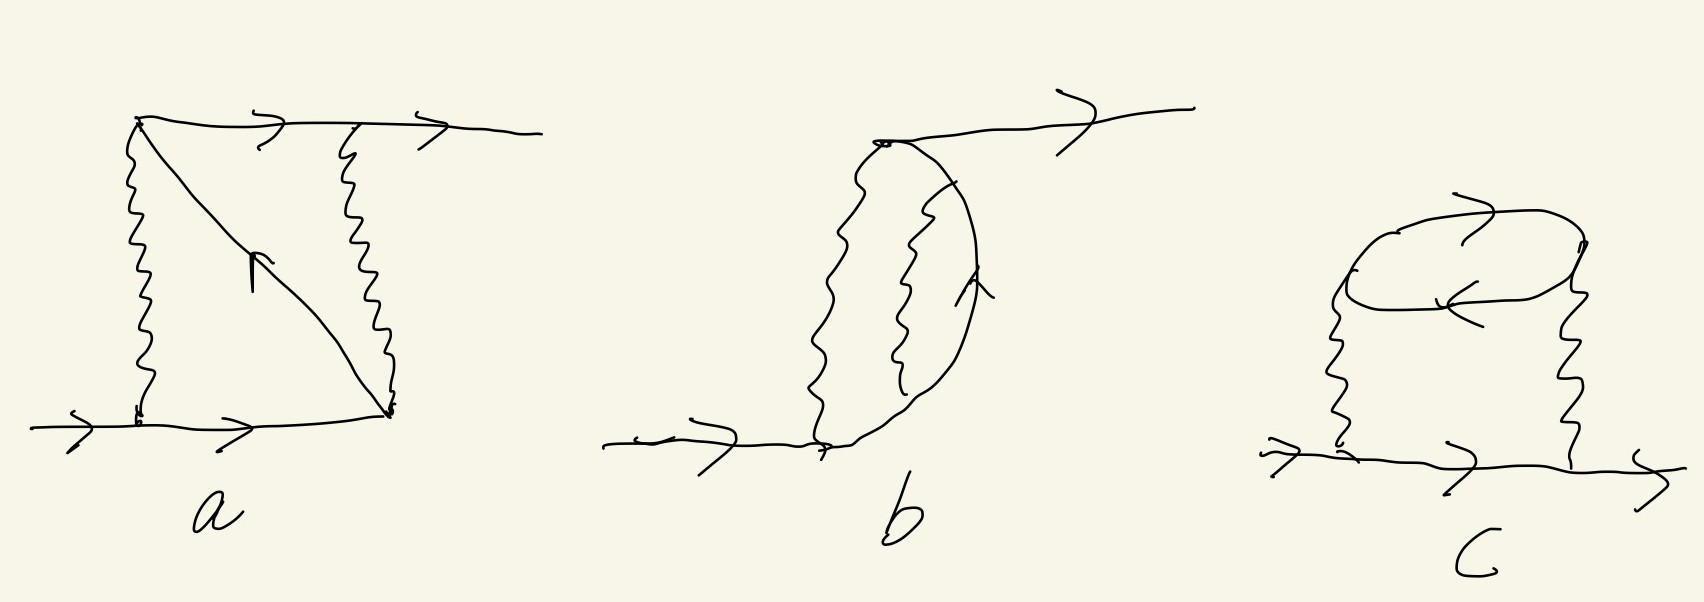
\includegraphics[width=0.8\linewidth]{./fig/fig5-2.jpg}
    \caption{Diagrame}%
    \label{fig:5.2}
\end{figure}

For Figure~\ref{fig:5.2}a, the self-energy contribution is
\begin{equation}
    \Sigma^{2a}(k) = \frac{1}{V^2\beta^2} \sum_{\bq \bq'} v_q v_{q'} \sum_{iq_n,iq_{ n'}} \cg^0(k+q) \cg^0(k+q') \cg^0(k+q+q')
\end{equation}
according \eqref{3.217} and calculation, we have
\begin{eqnarray}
    \Sigma^{2a}(k) &=& - \frac{1}{V^2} \sum_{\bq \bq'} \frac{v_q v_{q'}}{ik_n + \xi_{\bk+\bq+\bq'} - \xi_{\bk+\bq'} -\xi_{\bk+\bq} } \nonumber \\
    &=& \left[ \eta_F(\xi_{\bk+\bq'}) \left( \eta_F(\xi_{\bk+\bq}) - \eta_F(\xi_{\bk+\bq+\bq'})  \right) \right. \nonumber\\
    &+&\left. \eta_F(\xi_{\bk+\bq+\bq'})\left( 1- \eta_F(\xi_{\bk+\bq} \right) \right]
\end{eqnarray}
The self-energy of a particle is needed on the Fermi surface.
Set $k=k_F$ and $ik_n = \xi_{k_F} =k_F^2/2m - \mu = 0$.
The terms in the energy denominator largely cancel,
\begin{equation}
    \xi_\bk + \xi_{\bk+\bq+\bq'} - \xi_{\bk+\bq} - \xi_{\bk+ \bq'} = \frac{\bq \cdot \bq'}{m}   \label{5.44}
\end{equation}
The self-energy is
\begin{eqnarray}
    \Sigma^{2a}(k_F,0) &=& - \frac{(4\pi e^2)^2 m}{(2\pi)^6} \int \frac{d^3 q}{q^2} \int \frac{d^3 q'}{(q')^2} \frac{1}{\bq \cdot \bq'} \nonumber \\
    &\times& \{ \eta_F(\xi_{\bk+\bq'}) \left[ \eta_F(\xi_{\bk+\bq}) - \eta_F(\xi_{\bk+\bq+\bq'})  \right] + \dots  \} \label{5.45}
\end{eqnarray}
The quantity on the right is independent of the electron density.
The integral is convergent and give nonzero result.
It contribute the constant term in $E_c$.
With further calculation by Onsager, we have
\begin{equation}
    \Sigma^{2a} = \frac{1}{3} \ln(2) - \frac{3}{2\pi^2}  \zeta(3) = 0.0436
\end{equation}

\subsection{$\Sigma^{2b}$}
The second self-energy term involving two Coulomb lines is shown in Figure~\ref{fig:5.2}b, this contribution can be shown equal to zero.
Consider the summation of the similar diagrams, all terms may be summed by evaluating the exchange energy with an electron Green's function in the self-energy which includes the exchange energy.
This summation is given by the self-energy
\begin{equation}
    \Sigma'_x(k) = - \frac{1}{V\beta} \sum_{\bq,ik_n} v_q \cg(\bk+\bq,ik_n) \label{5.47}
\end{equation}
\begin{equation}
    \cg (\bk+\bq,ik_n) = \frac{1}{ik_n - \xi_{\bk+\bq} -\Sigma_x(\bk+\bq)} \label{5.48}
\end{equation}
where the Green's function has a self-energy due to exchange.

\chapter{Electrion-Phonon Interaction}

\section{Fr\"{o}hlich Hamiltonian}
The Fr\"{o}hlich Hamiltonian describes the interaction between a single electron in a solid and longitudinal optical phonons
\begin{align}
  \label{7.1}
  H &= \sum_{\mathbf{p}\sigma} \varepsilon_{\mathbf{p}} C^{\dagger}_{\mathbf{p}\sigma} C_{\mathbf{p}\sigma} + \omega_0 \sum_{\mathbf{q}} a^{\dagger}_{\mathbf{q}}a_{\mathbf{q}} + \sum_{\mathbf{pq}\sigma} \frac{M_{0}}{\sqrt{\nu}} \frac{1}{\abs{q}} C^{\dagger}_{\mathbf{p+q},\sigma} C_{\mathbf{p}\sigma} \left( a_{\mathbf{q}} + a^{\dagger}_{\mathbf{-q}} \right) \nonumber \\
  M_0 &=
\end{align}



%%% Local Variables:
%%% mode: latex
%%% TeX-master: "main"
%%% End:

chapter{Optical Properties of Solids}

\section{Wannier Excitons}\label{s9.2}
%
\subsection{The Model}
Exciton states play an extremely important role in the understand of interband transitions in semiconductors.
The word exciton is used to signify the modification of the \textit{absorption rate of phonons due the the Coulomb interaction between the electron and the valenec band hole}.

\begin{figure}[ht]
    \centering
    \begin{tikzpicture}
        \node at (-1.5,4.5) {a};
        \draw [->] (0,0) -- (0,4);
        \draw [->] (-1,0.2) -- (1,0.2);
        \node [below] at (1,0.2) {$k$};
        \draw (-1.5,0) .. controls (-0.25,2) and (0.25,2) .. (1.5,0);
        \draw (-1.5,4) .. controls (-0.25,2) and (0.25,2) .. (1.5,4);
        \draw (0,1.525) -- (1,1.525);
        \node [right] at (1,1.55) {$E=0$};
        \draw [->] (-1,0.9) -- (-1,3.1);
        \node at (3,4.5) {b};
        \draw [snake it] (3,0)--(3,2);
        \draw [middlearrow=latex] (3,2) -- (2,3);
        \draw [middlearrow=latex] (3,2) -- (4,3);
        \node [above] at (2,3) {$e^-$};
        \node [above] at (4,3) {$h^+$};
    \end{tikzpicture}
    \caption{Optical transition in a semiconductor between occupied valence band and empty conduction band for a direct transition. (a) Conventional band picture; (b) Wannier picture where the photon makes an electron-hole.}%
    \label{fig:9.6}
\end{figure}
%
The easiest case is shown in Fig.\ref{fig:9.6}(a), the interband transition is direct.
The valance band states are all filled and the conduction band states are all empty.
The vertical arrow show a possible interband transition which can occur when a photon is absorbed in the solid.
The valence state is shown as nondegenerate (except for spin) at $\bk=0$, although that is seldom the case; usually the band has an orbital degeneracy and is anisotropic.

\textit{The point of view in Fig.\ref{fig:9.6}(a) is a single-particle picture of the transition process}.
The transition rate for the absorption of photons is given by golden rule
\begin{eqnarray}
    A(\omega) &=& \frac{2\pi}{\hbar V} \sum_{\bk \bk'} \abs{ \bra{c,\bk'} \hat{\varepsilon} \cdot \bp \ket{v,\bk} }^2 \delta \left[\varepsilon_v(\bk) + \hbar \omega - \varepsilon_c(\bk') \right]      \label{9.73} \\
    \varepsilon_v(\bk) &=& - \frac{k^2}{2m_v},  ~ ~ ~ ~ \varepsilon_c(\bk) = E_g + \frac{k^2}{2m_c}  \label{9.74}
\end{eqnarray}
The energy zero is chosen to be the top of the valence band.
The matrix element is between the one-electron initial and final states.
The wave function are taken to be Bloch function $u_{\bk}(\br) \otimes\exp(i\bk \br)$.
For discussion reason assume the cell-periodic parts as independent of wave vector $\bk$, and assumed that the valance band has $p$ symmetry and conduction band has $s$ symmetry.
Then $u_v(\br)$ is a periodic orbital with angular momentum $l=1$, while $u_c(\br)$ is $l=0$.
With these approximations the optical matrix element is a constant except for wave vector conservation
\begin{eqnarray}
    \ket{v,\bk} &=& u_v(\br) \frac{e^{i\bk\br}}{\sqrt{V}} \label{9.75} \\
    \ket{c,\bk'} &=& u_v(\br) \frac{e^{i\bk'\br}}{\sqrt{V}} \label{9.76} \\
    \bra{c,\bk'} \hat{\varepsilon} \bp \ket{v,\bk} &\equiv& \hat{\varepsilon} \bp_{cv} \delta_{\bk\bk'} \label{9.77} \\
    \hat{\varepsilon}\bp &=& \frac{1}{V} \int_{cell} d^3 r u_c^* \hat{\varepsilon} \bp u_v  \label{9.78}
\end{eqnarray}
neglect the wave vector $\bq$ for photons since it is in the optical frequencies.
\begin{equation}
    A(\omega) = \abs{\hat{\varepsilon} \bp_{cv} }^2 \frac{(2\mu)^{3/2}}{2\pi} \sqrt{\hbar \omega - E_g} \Theta(\hbar \omega -E_g)   \label{9.79}
\end{equation}
with $\mu^{-1} = m_c^{-1} + m_v^{-1}$.
Equation \eqref{9.79} predicts that the absorption rate begins at the energy gap of semiconductor and rise as the square root of factor of optical frequency.
But this is not observed, in fact, the one-particle theory is totally inadequate.

Wannier observed that the interband transition in semiconductors was really a \textbf{two-particle process}, as in Fig.\ref{fig:9.6}(b).
In this new picture, the electron and hole are particles with charges of opposite sign, so that there is a Coulomb attraction $- \frac{^2}{\varepsilon_0 r}$ between them, where $\varepsilon_0$ is the static dielectric function.
The dielectric function is assumed to be a constant which is independent of the frequency.\footnote{This is a poor approximation, since most semiconductors are polar and dielectric function has significant dispersion at frequencies near the optical phonon frequencies, see \ref{s6.3}}
The attractive Coulomb interaction between the electron and hole can cause hydrogenic bound states between them.

The optical absorption rate for this process was calculated by Elliott. The final state of the system is described by a two-particle Sch{\"o}dinger equation
\begin{eqnarray}
    &&\Psi(\br_e,\br_h) = u_c(\br_e) u_v(\br_h) \Phi(\br_e,\br_h)     \label{9.82}    \\
    &&0 =\left[ - \frac{\hbar^2\nabla_e^2}{2m_c} - \frac{\hbar^2\nabla_h^2}{2m_v}  - \frac{e^2}{\varepsilon_0 \abs{\br_e-\br_h}} -E  \right] \Phi(\br_e,\br_h)   \label{9.83}
\end{eqnarray}
$\Phi(\br_e,\br_h)$ can be factored into relative $\br = \br_e-\br_h$ and center of mass coordinate $M=m_c+m_v$ in standard fashion
\begin{eqnarray}
    \mathbf{R} &=& \frac{m_c \br_e+m_v \br_h}{M}        \label{9.84} \\
    \Phi(\br_e,\br_h) &=& \frac{e^{i\mathbf{PR}}}{\sqrt{V}} \phi(\br)    \label{9.85} \\
    0 &=& \left( - \frac{\hbar^2}{2\mu} \nabla^2 - \frac{e^2}{\varepsilon_0 \br} -\varepsilon_r \right) \phi(\br)       \label{9.86} \\
    E &=& E_g + \varepsilon_r + \frac{P^2}{2M}  \label{9.87}
\end{eqnarray}
The center of mass motion is plane-wave-like, with a wave vector $\mathbf{P}$ which in optical experiments is equal to the photon wave vector.
This is usually small and set $\mathbf{P}=0$.
For relative energy $\varepsilon_r<0$, the two particles form bound hydrogenic states with energy $\varepsilon_r = \varepsilon_n = - \frac{E_R}{n^2} $.  For relative energy greater than zero, the form scattering states $\phi_\bk(\br)$.
Elliott showed that the optical transition rate depends on the relative wave function $br=0$.
Instead of \eqref{9.79}, the transition rate is
\begin{equation}
    A(\omega) = \frac{2\pi}{\hbar} \abs{\hat{\varepsilon} \bp_{cv}}^2 \sum_j \abs{\phi_j(0)}^2 \delta(\hbar \omega - E_g -\varepsilon_j)  \label{9.88}
\end{equation}
The summation $j$ run over the bound and continuum states.

The relative motions of electron and hole are in s-wave hydrogenic state, either bound or unbound, because of the angular momentum selection rule.
The one-unit change in $l$, in the photon absorption, is take by the change of band symmetry, and the relative motion is not permitted any additional angular momentum.
For $s$ states, the bound states have an amplitude given by the principal quantum number $n$ and the Bohr radius $a_0$,
\begin{equation}
    \phi_n(0) = \frac{1}{\sqrt{\pi a_0^3 n^3}} \label{9.89}
\end{equation}
For continuum states, with energy $\varepsilon_k = \frac{k^2}{2\mu} $, the relative wave function at the origin is
\begin{equation}
    \psi_{k,l=0}(0) = \frac{2\pi \eta}{V \left[2- e^{-2\pi \eta} \right]}
\end{equation}
where $\eta^{-1} = k a_0$.
Then \eqref{9.89} predicts that the absorption is a constant in frequency at the energy gap $E_g$, and does not rise with a square root dependence.
The absorption function now have a few sharp, distinct exciton lines at low frequency correspond to $1s$, $2s$, etc.
These absorption bands are very strong, and all the light is attenuated before trasversing the sample.
At higher frequencies, the $ns$ stats are closer in frequency and are broadened and merges with the continuum absorption which starts at $\hbar \omega = E_g$.

\subsection{Solution by Green's Functions}


\chapter{Superconductivity}
The theory of superconductivity was formulated by Bardeen, Cooper, and Schrieffer (1957) and is called the BCS theory.
It very successfully describes the superconducting properties of weak superconductors, such as aluminum, which are weak because of the small strength of electron-phonon interaction.
Further refinement of the theory have led to strong coupling theory of Eliashberg, which describes the properties of superconductor lead.
The distinction is roughly determined by the value of the electron-phonon mass enhancement factor $\lambda$ shown by McMillan.

The basic idea of BCS theory is that the electrons in the metal form bound pairs.
This bound states of electron pairs are not described by simple orbitals such as hydrogen atom.
The pair state and entire ground state of the superconductor requires a many-body description.

Fr{\"o}hlich was the first to realize that electrons could interact by exchanging phonons and that this interaction could be attractive.
Another piece in theoretical puzzle was supplied by Schafroth, who shown that a charged boson gas, when undergoing a Bose-Einstein condensation would exhibit many of superconducting properties such as Meissner effect.
In the BCS theory, the electron pairs behave in some respects as bosons.

\section{Cooper Instability} \label{s10.1}
Cooper pointed out that the ground state of a normal metal was unstable at zero temperature.
A normal metal is defined as one which is neither superconducting nor magnetic.
The demonstration of an instability does not provide a description of superconducting state, but it suggest that the instability was caused by the scattering between pairs of electrons, where the scattering potential is the exchange of phonons.

The scattering process as shown \ref{fig:10.1}.
\begin{figure}[ht]
    \centering
    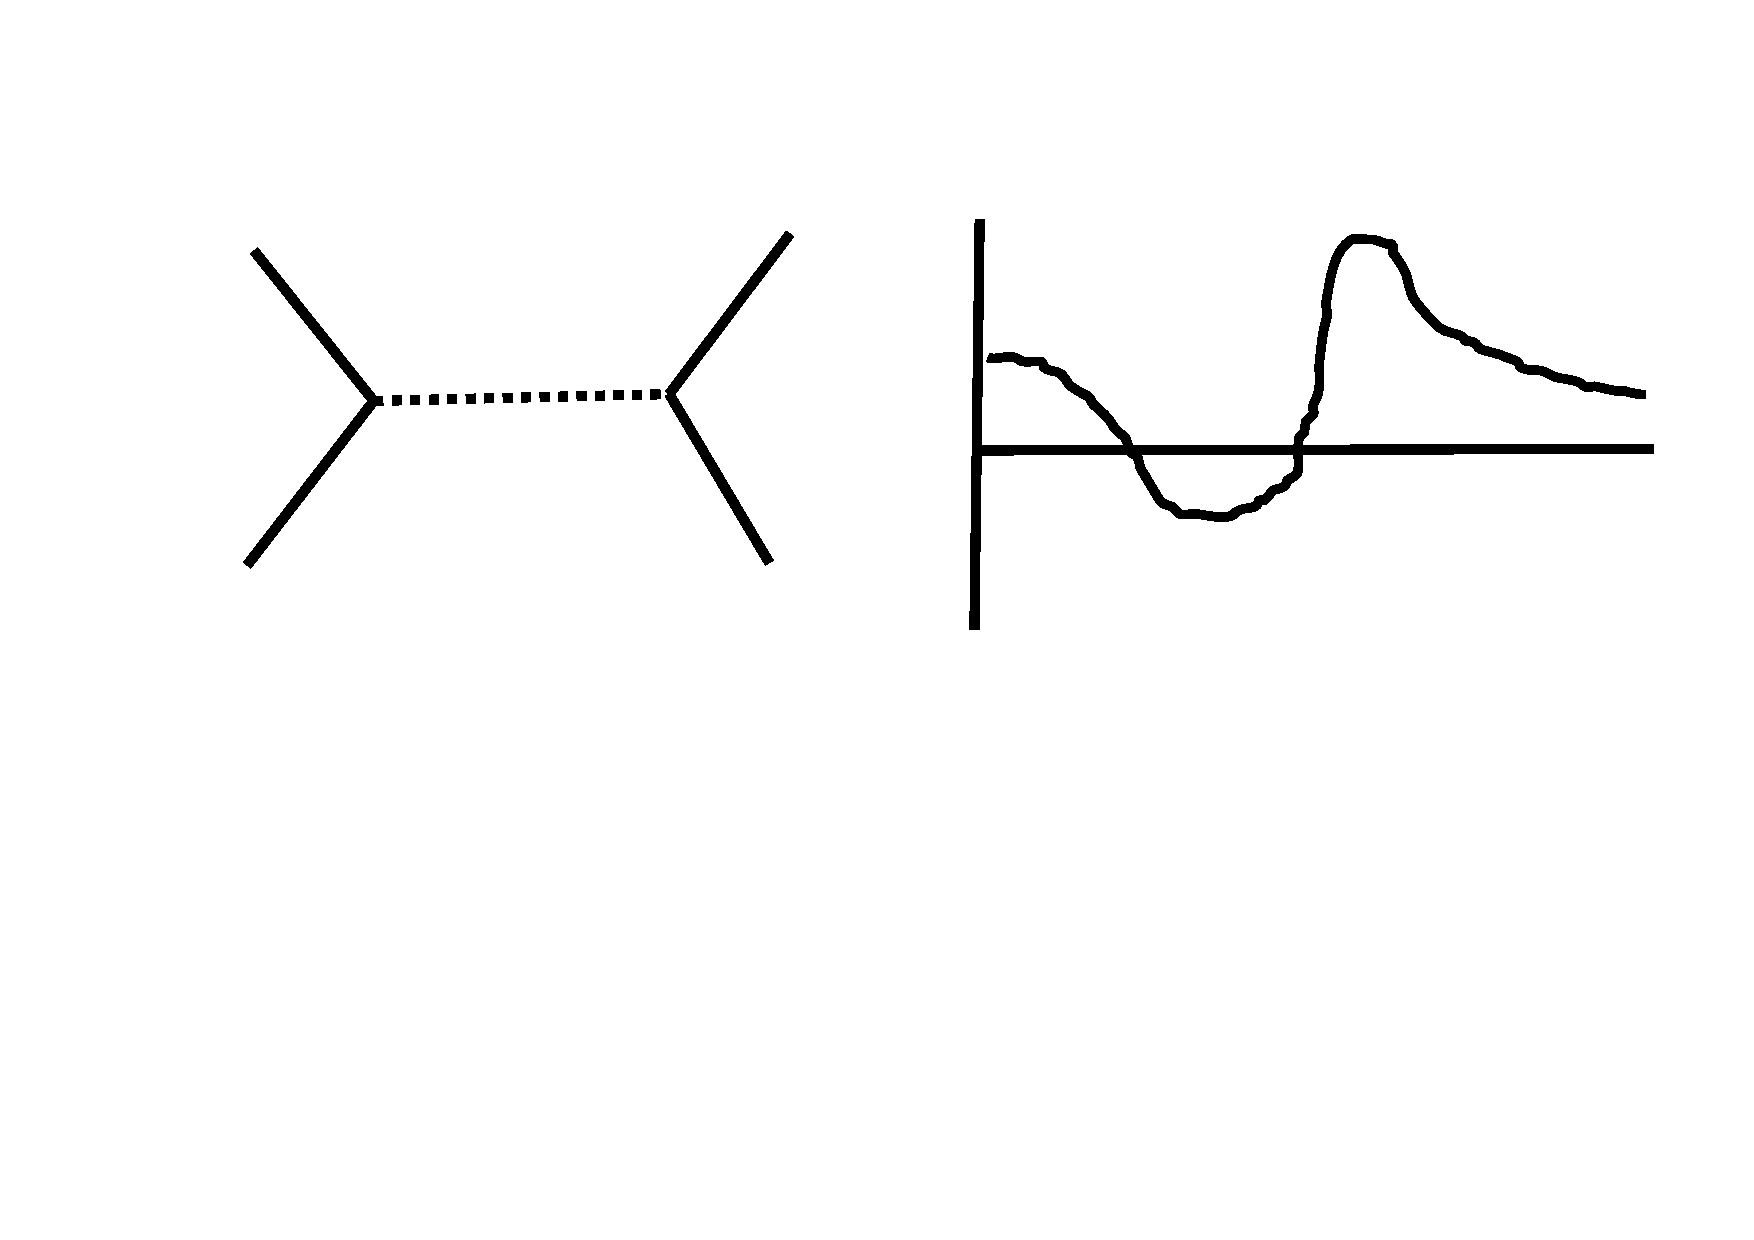
\includegraphics[width=0.8\linewidth]{./fig/fig10_1.pdf}
    \caption{Scattering process and potential}%
    \label{fig:10.1}
\end{figure}
The screened interaction between two electrons was derived before as
\begin{equation}
    V_s(\bq,\omega) = \frac{v_q}{\varepsilon(\bq,\omega)}  + \frac{2\omega \lambda M^2_\bq}{\varepsilon(\bq)^2 \left[ \omega^2 - \omega_\lambda(\bq)^2\right]}  \label{10.1}
\end{equation}
The first is the screened Coulomb interaction.
The theory of superconductivity is applied at low temperatures, where the energy exchanged between particles, while scattering, is also low.
The requirements of crystal stability require that this interaction be repulsive at zero frequency.

The second term in \eqref{10.1} is the screened electron-phonon interaction.
It is on the average weaker than the repulsive Coulomb interaction.
However, for frequency near to Debye $(\omega <\omega_D)$ the energy denominator becomes small and negative, which causes a relatively large interaction over this narrow range of frequency.
It may be possible for two electrons to bind if they can construct a relative wave function which selectively uses the frequency region which is attractive.

For simplicity instead of \eqref{10.1} use a interaction model
\begin{equation}
    V_s(\bq,\omega) =
    \begin{cases}
        -V_0 ~ ~&  \abs{\xi_q}<\omega_D \\
        0 & \abs{\xi_q}>\omega_D
    \end{cases} \label{10.2}
\end{equation}
This potential is constant and attractive up to a cutoff energy which is of the order of the Debye energy $\omega_D$ of the solid.

The Cooper's model of a normal metal at low temperature was a free-electron system.
The electrons are allowed to have a weak attractive interaction as in \eqref{10.2}.
Consider the mutual scattering of two electrons.
Assume they initially have states of equal and opposite momentum, $\bk$ and $-\bk$.
It is also assumed the particles have opposite spin that exchange scattering does not occur\footnote{P298 Hatree fock approximation}.
The interaction potential does not flip the electron spin and the spin states are preserved in the scattering process.

\begin{figure}[ht]
    \centering
    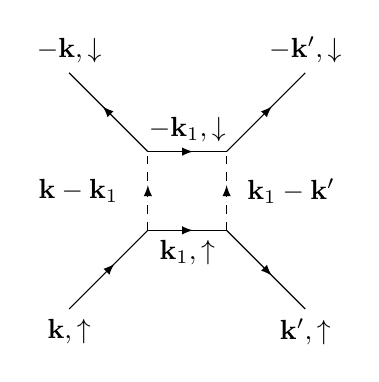
\begin{tikzpicture}
        \draw [middlearrow=latex] (0,0) -- (1,1);
        \draw [middlearrow=latex,dashed] (1,1) -- (1,2);
        \draw [middlearrow=latex] (1,2) -- (0,3);
        \draw [middlearrow=latex] (1,2) -- (2,2);
        \draw [middlearrow=latex] (1,1) -- (2,1);
        \draw [middlearrow=latex,dashed] (2,1) -- (2,2);
        \draw [middlearrow=latex] (2,2)--(3,3);
        \draw [middlearrow=latex] (2,1)--(3,0);
        \node [right,below] at (0,0) {$\bk,\uparrow$};
        \node [left] at (0.75,1.5) {$\bk-\bk_1$};
        \node [left,above] at (0,3) {$-\bk,\downarrow$};
        \node [above] at (1.5,2) {$-\bk_1,\downarrow$};
        \node [below] at (1.5,1) {$\bk_1,\uparrow$};
        \node [left,below] at (3,0) {$\bk',\uparrow$};
        \node [left] at (3.5,1.5) {$\bk_1-\bk'$};
        \node [left,above] at (3,3) {$-\bk',\downarrow$};
    \end{tikzpicture}
    \caption{Scattering event between two electron lines from left to right.}%
    \label{fig:10.2}
\end{figure}
In Figure \ref{fig:10.2} show a double scattering event between two electron lines which are moving in the same direction in time.
This process is the scattering in the second \textbf{Born approximation}, where the firs Born approximation is shown in Fig.\ref{fig:10.1}.
The effective scattering in the first and second Born approximation is
\begin{equation}
    V_{eff}(\bk-\bk') = V(\bk-\bk') + \int \frac{d^3 k_1}{(2\pi)^3} \frac{V(\bk-\bk_1) V(\bk_1- \bk')}{2\xi_\bk - 2 \xi_{\bk_1}} \left( \left[1-\eta_F(\xi_{\bk_1}) \right] \left[ 1- \eta_F(\xi_{\bk_1}) \right] - \eta_F(\xi_{\bk_1})^2 \right)   \label{10.3}
\end{equation}
The second term on the right is the contribution of Fig.\ref{fig:10.2}.
The denominator contains the initial state energy minus the intermediate state energy.
The factors $\left[ 1- \eta_f(\xi_{k_1})\right]^2 -\eta_F(\xi_{\bk_{1}})^2 = 1-2\eta_F(\xi_{\bk_{1}})$, which occur because the two particle can scatter into the state when they are not occupied.
The term $\eta_F(\xi_{\bk_1})^2$ represents the scattering back into this state, $\ket{\bk_1,\uparrow } \to \ket{\bk,\uparrow}$, since the result depends upon the net scattering.
What is left are the remaining factors $1-2\eta_F(\xi_{\bk_1})$, these occupation factors play a crucial role in the theory and are the cause of instability.
\marginnote{
    To under the \eqref{10.3}, the correlation operator looks like this
    \begin{equation}
        \langle \psi(t_1) \psi^\dagger(t_2) \psi(t_3) \psi^\dagger(t_4) S \rangle \nonumber
    \end{equation}
    where $S$ is the all possible interaction, like Green's function.
    The 'Dyson' equation looks
}
    \begin{marginfigure}
        \begin{tikzpicture}
            \draw [->] (0,0)--(0,1);
            \draw [->] (1,0)--(1,1);
            \draw [dashed] (0,0.45) -- (1,0.45);
            \draw [dashed] (0,0.55) -- (1,0.55);
            \draw [dashed] (0,-1.45) -- (1,-1.45);
            \draw [dashed] (0,-1.55) -- (1,-1.55);
            \node at (1.5,-1.5) {$ = \emptyset+$};
            \draw [dashed] (2,-1.5)--(3,-1.5);
            \draw [dashed] (2,-2)--(3,-2);
            \draw [dashed] (2,-3)--(3,-3);
            \node at (1.5,-2.5) {$+$};
            \draw [middlearrow=latex] (2,-3)--(2,-2);
            \draw [middlearrow=latex] (3,-3)--(3,-2);
        \end{tikzpicture}
    \end{marginfigure}
\marginnote{
    The Green function of election gives the different combination of distribution function.
}


The integral in \eqref{10.3} may be evaluated.
The key is that the interaction acts only over a small energy interval near the Fermi energy.
Over this Debye energy window, the electron density of states in most metal is nearly constant.
One can change the integration variable
\begin{equation}
    \int \frac{d^3k_1}{(2\pi)^3} = \int d\xi_1 N(\xi_1)
\end{equation}
and treat $N(\xi\approx 0) \equiv N_F$ as an constant. At zero temperature the result is $(\xi_{\bk_1} = \xi_1)$
\begin{equation}
    V_{eff}(\bk-\bk') = V(\bk-\bk') + N_F V_0^2 \int_{-\omega_D}^{\omega_D} d\xi_1 \frac{\frac{1}{2} - \eta_F(\xi_1)}{\xi-\xi_1} \label{10.4}
\end{equation}
The factor $1/2$ does not cause any singularity and may be ignored, then in zero temperature
\begin{equation}
    \int_{-\omega_D}^{\omega_D} d\xi_1 \frac{\eta_F(\xi_1)}{\xi-\xi_1} = -\ln \left( \frac{\xi}{\omega_D}  \right) \label{10.5}
\end{equation}
and
\begin{equation}
    V_{eff} = -V_0 \left[ 1- N_F V_0 \ln\left( \frac{\xi}{\omega_D} \right) \right] \label{10.6}
\end{equation}
The term $-N_F V_0 \ln (\xi/\omega_D)$ is regarded as the \textbf{vertex correction} which results from the additional scattering between electrons.
This scattering become very large for electrons near the Fermi energy.

Further insight is gained by considering the sum of diagrams like these.
Each additional interaction (dashed line) causes two more Green's function which are going parallel in the intermediate state.
Each new set of intermediate stats has the same type of integrand, so that a term with $(n+1)$ ladder diagrams gives a net contribution of
\begin{equation}
    -V_0 \left[ -N_F V_0 \ln \left( \frac{\xi}{\omega_D} \right) \right]^n      \label{10.7}
\end{equation}
The summation of these terms produces the series
\begin{eqnarray}
    V_{eff} &=& -V_0 \sum_{N=0}^\infty \left[ -N_F V_0 \ln \left( \frac{\xi}{\omega_D} \right) \right]^n \nonumber \\
    &=& - \frac{V_0}{1+N_F V_0 \ln \left( \xi/\omega_D \right)}  \label{10.9}
\end{eqnarray}
The denominator equals zero at ($V_{eff}=0$)
\begin{equation}
    \xi_0 = \omega_D \exp \left[ - \frac{1}{N_F V_0} \right]    \label{10.10}
\end{equation}
This $\xi_0$ gives a pole in \eqref{10.9}.
In the vicinity of $\xi_0$ can be approximated by using $\xi = \xi_0 + \left( \xi - \xi_0 \right)$ and the scattering has a pole
\begin{eqnarray}
    V_{eff} &=& - \frac{1}{N_F} \frac{1}{\ln(\xi/\xi_0)} = - \frac{1}{N_F} \frac{1}{\ln \left[ 1 + (\xi-\xi_0)/\xi_0 \right]}   \nonumber \\
    &\approx&- \frac{\xi_0}{N_F(\xi- \xi_0)}     \label{10.11}
\end{eqnarray}
This pole is sufficient to cause the instability.
\begin{figure}[ht]
    \centering
    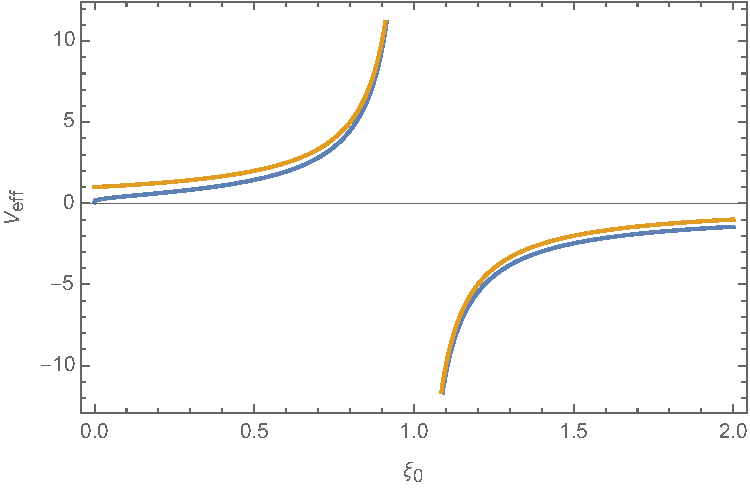
\includegraphics[width=0.55\linewidth]{./fig/fig_eq_10_11.pdf}
    \caption{The behaviour of $V_{eff}$ as the function of $\xi_0$. The yellow line is the approximation one.}%
    \label{fig:eq_10_1}
\end{figure}
The electrons near the Fermi energy will interact with their pair on the opposite side of the Fermi sea.
The mutual scattering produces a pole in the scattering amplitude, which will make the pair of electrons try to bind together.
The entire electron pairs are doing this simultaneously, so that the entire metal undergoes a phase transition.
The existence of this pole depended on the sharpness of the electron distribution.
If all the electrons near the Fermi energy become paired, one must reconsider whether this sharp distribution still exits.
A theory of superconductivity must self-consistently determine the properties of bound electron pairs.

Another way to describe the instability is as a function of temperature.
It enters into the electron distribution $\eta_F$ by changing the step function into a smooth function with an energy width of several $k_B T$.
By expressing the \eqref{10.5} as
\begin{equation}
    \int_{-\omega_D}^{\omega_D} d\xi_1 \frac{\eta_F(\xi_1)}{\xi-\xi_1} \approx  - \frac{1}{2} \ln \left[ \frac{\xi^2 + (k_B T)^2}{\omega_D^2}  \right] \label{10.12}
\end{equation}
Summation of all the ladder diagrams and the effective potential have the form
\begin{equation}
    V_{eff} = - \frac{V_0}{1+ N_F V_0 \ln \left[ \sqrt{\xi^2 + (k_BT)^2}/\omega_D  \right]}     \label{10.13}
\end{equation}
At zero energy, $\xi=0$, $V_{eff}$ becomes singular when the temperature is lower to the critical temperature $T_c$
\begin{equation}
    k_B T_c = \omega_D \exp \left[ - \frac{1}{N_F V_0} \right]  \label{10.14}
\end{equation}

The theory of Cooper instability should be compared, for example, with the ordinary binding of two isolated particles.
If two particles are isolated, they do not have to obey the statistics of a collection of identical particles.
Then the scattering theory does not contain any of the occupation factors. all states may be used as intermediate state since there are no other particles.
In theory of Wannier excitons \ref{s9.2}, the multiple scattering theory may be described by a vertex function
\begin{equation}
    \Gamma(\bk,\bk') = V(\bk-\bk') + \int \frac{d^3 k_1}{(2\pi)^3} \frac{V(\bk-\bk_1) \Gamma(\bk_1,\bk')}{2\xi_\bk - 2\xi_{\bk_1}}  \label{10.16}
\end{equation}
The solution to this vertex function is equivalent to solving the two-particle Schr{\"o}dinger equation in relative coordinates
\begin{equation}
    \left[- \frac{1}{2m} \left(\nabla_1^2 + \nabla_2^2 \right) + V(\br_1 -\br_2) -E \right] \psi(\br_1,\br_2) = 0   \label{10.17}
\end{equation}
The problem is factored into the relative and center of mass motions
\begin{eqnarray}
    \br &=& \br_1 - \br_2, ~ ~ ~ \psi(\br_1,\br_2) = e^{i \bp \cdot \mathbf{R}} \phi(\br) \label{10.18}\\
    \mathbf{R} &=& \frac{1}{2} (\br_1 + \br_2), ~ ~ ~ E= \frac{p^2}{2m} + \varepsilon   \label{10.19} \\
    &&\left[ - \frac{\nabla^2}{m} + V(\br) - \varepsilon \right] \phi(\br) = 0 \label{10.20}
\end{eqnarray}
The center of mass motion is plane wave, and the relative motion becomes a one-body problem.
Without the occupation factors, the relative scattering of two particles by an instantaneous potential is a trivial problem.
When bound states occur, they are at negative binding energy in the relative coordinates, $\varepsilon<0$.
This behaviour is great contrast to the Cooper instability, where the pole occurs at small negative energy relative the to $E_F$, so the pole is at a positive energy $E_F-\xi_0$.
The two electrons cannot really bind at that energy, since their net energy is positive.
\textit{The instability occurs because it appears to them as if they should bind, although if they tried, they would find they could not.}
The role of the occupation factors in the argument of the scattering integral is what moved the apparent pole out to the Fermi energy.\footnote{The reason electrons must be paired with opposite momentum, P633}

\subsection{BCS Theory}
The basic feature of the BCS theory is that pairing occurs between electrons in states with opposite momentum ans opposite spins.
The two spins are combined into a spin singlet, with $S=0$.
We will assume this spin arrangement during the discussion.

The pairing of electrons in the BEC theory mus cause correlations in the relative motion.
The pairing is describe by introducing a new correlation function, similar to Green's function, for particles of opposite spin.
They are
\begin{eqnarray}
    \cg(\bp, \tau-\tau') &=& - \langle T_\tau C_{\bp\sigma} (\tau) C^\dagger_{\bp\sigma}(\tau') \rangle \nonumber \\
    \cf(\bp, \tau-\tau') &=& \langle T_\tau C_{-\bp\downarrow}(\tau) C_{\bp\uparrow}(\tau') \rangle \label{10.31} \\
    \cf^\dagger (\bp,\tau-\tau') &=& \langle T_\tau C^\dagger_{\bp\uparrow}(\tau) C^\dagger_{-\bp\downarrow}(\tau') \rangle \nonumber
\end{eqnarray}
The Green's function $\cg$ has the same definition as usual, although it has a different algebraic form in the superconducting state.
The $\cf$ functions are identically zero in the normal state.
A basic feature of the BCS ground state wave function is that it is composed of a superposition of electronic states containing a different number of electrons.
One need to find a self--consistent equation for the correlation function and its conjugate.

To provide the simplest possible model of BCS theory, assume a Hamiltonian of the form
\begin{equation}
    H = \sum_{\bp \sigma} \xi_\bp C^\dagger_{\bp\sigma} C_{\bp\sigma}  +  \frac{1}{2V} \sum_{\bq \bp \bp' s s'} V(q) C^\dagger_{\bp+\bq,s} C^\dagger_{\bp'-\bq,s'} C_{\bp' s'} C_{\bp s}   \label{10.35}
\end{equation}
The interaction potential $V(q)$ between electrons is taken to have the form in \eqref{10.2}, which is an attractive constant $V(q) = - V_0$ over a range of energies within a Debye energy of the Fermi surface.
With this Hamiltonian, a set of self--consistent equations will be derived for the Green's functions $\cg$, $\cf$ and $\cf^\dagger$.
Using the equation of the motion
\begin{equation}
    \frac{d}{d\tau} C_{\bp\sigma} (\tau) = \left[H, C_{\bp\sigma} \right] = -\xi_\bp C_{\bp\sigma} - \frac{1}{V} \sum_{\bq \bp' s'} V(q) C^\dagger_{\bp'-\bq,s'} C_{\bp's'} C_{\bp-\bq,\sigma}  \label{10.36}
\end{equation}
From the definition of the $\tau$--order product, the first derivative of the equation for the Green's function is
\begin{equation}
    \frac{\partial}{\partial \tau} \cg(\bq,\tau-\tau') = - \delta(\tau-\tau') - \langle T_\tau \left[ \frac{\partial}{\partial \tau} C_{\bp\sigma}(\tau) \right] C^\dagger_{\bp\sigma}(\tau') \rangle   \label{10.38}
\end{equation}
Using the result \eqref{10.36} for the derivative gives
\begin{eqnarray}
    &~&\left( - \frac{\partial}{\partial \tau}  - \xi_p \right) \cg(\bq,\tau-\tau') + \frac{1}{V} \sum_{\bq\bp's} V(q) \nonumber \\
    &~& \times \langle T_\tau C^\dagger_{\bp'-\bq,s'} C_{\bp's'}(\tau) C_{\bp-\bq,\sigma}(\tau) C^\dagger_{\bp\sigma}(\tau') \rangle = \delta(\tau-\tau')    \label{10.40}
\end{eqnarray}
There are many ways of doing the pairing.
One simplification is to assume that long--wavelength phonons give a zero potential, so that $V(\bq=0) = 0$.
For a normal metal, there would only remain the pairing $\delta_{\bp\bp'} \delta_{s'\sigma} \eta_{\bp-\bq} \cg(\bp,\tau-\tau')$ which gives the exchange energy.
This pairing occurs in the superconductor as well but is not the only term.
The pairing which include the $\cf$ function must pay attention to the spin variables.
The combination $\sigma= - s' = \uparrow$ gives
\begin{equation}
    \langle T_\tau C^\dagger_{\bp'-\bq,s'} C_{\bp's'}(\tau) C_{\bp-\bq,\sigma}(\tau) C^\dagger_{\bp\sigma}(\tau') \rangle = - \delta_{\sigma,-s'} \delta_{\bp',-\bp+\bq} \cf(\bp-\bq,0) \cf^\dagger(\bp,\tau'-\tau) \label{10.42}
\end{equation}
where the sign change result from an odd number of operator rearrangements.
Similarly, the choice $\sigma = - s' = \downarrow$ gives
\begin{equation}
    \langle T_\tau C^\dagger_{\bp'-\bq,s'} C_{\bp's'}(\tau) C_{\bp-\bq,\sigma}(\tau) C^\dagger_{\bp\sigma}(\tau') \rangle = - \delta_{\sigma,-s'} \delta_{\bp',-\bp+\bq} \cf(-\bp+\bq,0) \cf^\dagger(-\bp,\tau-\tau') \label{10.44}
\end{equation}
\textit{These two results are identical, since later it is shown that $\cf$ and $\cf^\dagger$ do not depend on the sign of the arguments either momentum or $\tau$}.
The last term in \eqref{10.40} gives the expression
\begin{eqnarray}\label{10.45}
    &~& \frac{1}{V} \sum_{\bq\bp's} V(q)  \langle T_\tau C^\dagger_{\bp'-\bq,s'} C_{\bp's'}(\tau) C_{\bp-\bq,\sigma}(\tau) C^\dagger_{\bp\sigma}(\tau') \rangle    \\ 
    &=& \frac{1}{V} \sum_{\bq} V(q) \left[\cg(\bp,\tau-\tau')\eta_{\bp-\bq} - \cf(\bp-\bq,0)\cf^\dagger(\bp,\tau-\tau') \right] \nonumber
\end{eqnarray}
The first term is the exchange self--energy of the electron due to the phonon induced interaction between electrons.
A careful investigation shows that this self--energy does not change much between the normal and superconducting states.
The self--energy of the electrons, from phonons, causes a change in the electron effective mass given by the parameter $\lambda$.
This effect is not large in weak superconductors, so it may be \textbf{ignored}.
In metals where $\lambda$ is large, the superconducting state can be expected to significantly alter the properties of electrons near the Fermi surface where strong coupling theory is needed.

In the second term of \eqref{10.45} there arises the combination of factors which are defined as
\begin{equation}
    \Delta (\bp) = - \frac{1}{V} \sum_\bq V(q) \cf(\bp-\bq,\tau=0)  \label{10.46}
\end{equation}
The quantity $\Delta(\bp)$ is the gap function in the BCS theory.
This quantity is defined to be positive, since the right--hand side of the definition is positive, with an attractive potential $V(q)<0$.
So the \eqref{10.40} gives
\begin{equation}
    \left( - \frac{\partial}{\partial \tau} - \xi_p \right) \cg(\bp,\tau-\tau') + \Delta(\bp) \cf^\dagger (\bp,\tau-\tau') = \delta(\tau-\tau') \label{10.47}
\end{equation}


\chapter{Appendix: Complex analysis}

\section{Residue}
In complex analysis, the \textbf{residue} is a complex number proportional to the contour integral of a meromorphic function along a path enclosing one of its singularities.

\subsection{Definition}
The residue of a \href{https://en.wikipedia.org/wiki/Meromorphic_function}{meromorphic function} $f$ at an isolated singularity $a$, denoted as $\Res(f,a)$, is the unique value $R$ such tat $f(z)-R/(z-a)$ has an analytic antiderivative in a punctured disk $0<\abs{z-a}<\delta$.

Alternatively, residues can be calculated by Laurent series expansions, and one can define the residue as the coefficient $a_{-1}$ of a Laurent series.

\subsection{Examples}
\textbf{Eaxmple.1}\\
Computing the residue of a monomial,
\begin{equation*}
  \oint_C z^k dz
\end{equation*}
Since path integral computations are homotopy invariant, let $C$ be the radius of $1$, and $dz \to d(e^{i\theta}) = ie^{i\theta} d\theta$.
The result is
\begin{equation*}
  \oint_C z^k dz = \int_0^{2\pi} i e^{i(k+1)\theta} d\theta =
  \begin{cases}
    2\pi i ~ ~ ~ &(k=-1) \\
    0 ~ ~ ~ &(\mathrm{otherwise})
  \end{cases}
\end{equation*}
\textbf{Example.2}
Consider the contour integral, where $C$ is some simple closed curve about $0$.
\begin{eqnarray*}
  &&\oint_C \frac{e^z}{z^5}dz  \\
  &=&\oint_C \frac{1}{z^5}(1+z+\frac{z^2}{2!}+\frac{z^3}{3!}+\dots)dz \\
  &=& \oint_C \frac{1}{4! z} dz \frac{\pi i}{12}
\end{eqnarray*}
The last formula is based on the previous result.

\subsection{Calculating residues}
For residue theorem,
\begin{equation*}
  \Res(f,c) = \frac{1}{2\pi i} \oint_\gamma f(z) dz
\end{equation*}
where $\gamma$ traces out a circle around $c$ in a counterclockwise manner.

\textbf{Removeable singularities}\\
If function $f$ can be continued to a holomorphic function on the whole disk, then $\Res(f,c)=0$.
The converse is not generally true.

\textbf{Simple poles}\\
At a \href{https://en.wikipedia.org/wiki/Zeros_and_poles}{simple pole} $c$, the residue of $f$ is given by
\begin{equation*}
  \Res(f,c) = \lim_{z\to c}(z-c)f(z)
\end{equation*}
It may be that the function $f$ can be expressed as a quotient of two function, $f(z)=\frac{g(z)}{h(z)}$, where $g$ and $h$ are \href{https://en.wikipedia.org/wiki/Holomorphic_function}{holomorphic functions} in a neighborhood of $c$, with $h(c)=0$ and $h'(c)\neq 0$.
  In such case, \href{https://en.wikipedia.org/wiki/L%27H%C3%B4pital%27s_rule}{L'H\^{o}pital's rule} can be use to simplify the formula to
\begin{equation*}
  \Res(f,c)= \frac{g(c)}{h'(c)}
\end{equation*}
More generally, if $c$ is a pole of order $n$, the residue of $f$ around $z=c$ can be found by the formula
\begin{equation*}
  \Res(f,c)=\frac{1}{(n-1)!} \lim_{z\to c} \frac{d^{n-1}}{dz^{n-1}} \left[(z-c)^n f(z) \right]
\end{equation*}

In general, the residue at infinity is given by
\begin{equation*}
  \Res(f(z),\infty) = - \Res(\frac{1}{z^2}f(\frac{1}{z}),0)
\end{equation*}

\textbf{Series methods}\\
If parts or all of a function can be expand into a Taylor series or \href{https://en.wikipedia.org/wiki/Laurent_series}{Laurent series}, which may be possible if the parts or the whole of the function has a standard series expansion, the calculating the residue is significantly simpler than by other methods.

Considering the integral
\begin{equation*}
  f(z)= \frac{\sin z}{z^2-z}
\end{equation*}
where $z=0$ is the removable singularity and the residue at this point is $0$.
The Taylor expansion gives, at point $z=1$,
\begin{eqnarray*}
    \sin z &=& \sin 1 + \cos 1 (z-1) + \frac{-\sin 1}{2!}(z-1)^2 + \dots \\
    \frac{1}{z} &=& \frac{1}{(z-1)+1} = 1 -(z-1) +(z-1)^2 -(z-1)^3 + \dots \\
\end{eqnarray*}
Multiplying those two series and introducing $1/(z-1)$ gives
\begin{equation*}
  \frac{\sin z}{z(z-1)} = \frac{\sin 1}{z-1} + (\cos 1 - \sin 1) + (z-1)(-\frac{\sin 1}{2!} - \cos 1 + \sin 1) + \dots
\end{equation*}
So the residue of $f(z)$ at $z=1$ is $\sin 1$.

\section{Sokhotski-Plemelj theorem}
Let $f$ be a complex-valued function which is defined and continuous on the real line and let $a$ and $b$ be real constants with $a<0<b$, then
\begin{equation*}
  \lim_{\varepsilon\to 0^+} \int_a^b \frac{f(x)}{x\pm i\varepsilon}dx = \mp i\pi f(0) + \mathcal{P} \int_a^b \frac{f(x)}{x} dx,
\end{equation*}
where $\mathcal{P}$ denotes the \href{https://en.wikipedia.org/wiki/Cauchy_principal_value}{Cauchy principal value}.

One important relation is for the Green's functions,
\begin{equation*}
  \frac{1}{\omega + E_n - E_m + i\delta} = \mathcal{P} \frac{1}{\omega + E_n -E_m} - i\pi \delta(\omega +E_n -E_m)
\end{equation*}

\section{Kramers-Kronig relations}
The Kramers-Kronig relations are bidirectional mathematical relations, connection the real and imaginary parts of any complex funtion that is analytic in the upper half-plane.
The relations are often used to compute the real part from the imaginary part of response functions in physical systems, because for stable system, causality implies the condition of analyticity and conversely, analyticity implies causality of the corresponding stable physical system.

Let $\chi(\omega) = \chi_1(\omega) + i \chi_2(\omega)$ be a complex function of the complex variable $\omega$, where $\chi_1$ and $\chi_2$ are real.
Suppose this function is analytic in the upper half-plane of $\omega$ and vanishes like $1/\abs{\omega}$ or faster as $\abs{\omega}\to \infty$.
The Kramers-Kronig relations are given by
\begin{equation*}
  \chi_1(\omega) = \frac{1}{\pi} \mathcal{P}\int_{-\infty}^\infty \frac{\chi_2(\omega')}{\omega'-\omega} d\omega'
\end{equation*}
and
\begin{equation*}
  \chi_2(\omega) = -\frac{1}{\pi} \mathcal{P} \int_{-\infty}^\infty \frac{\chi(\omega')}{\omega'-\omega} d\omega'
\end{equation*}
alternatively, we have the following formulas
\begin{eqnarray*}
    \chi_1(\omega) &=& \frac{2}{\pi} \mathcal{P} \int_0^\infty \frac{\omega' \chi_1(\omega')}{\omega'^2-\omega^2} d\omega' \\
    \chi_2(\omega) &=& -=\frac{2\omega}{\pi} \mathcal{P} \int_0^\infty \frac{\chi_1(\omega')}{\omega'^2 -\omega^2} d\omega'
\end{eqnarray*}


\bibliography{mybib}{}
\bibliographystyle{abbrv}
\end{document}
